\documentclass[11pt, onecolumn]{report}
%%% PAGE DIMENSIONS
\usepackage{geometry} % to change the page dimensions
\geometry{a4paper, columnsep=5mm}
\setlength{\parindent}{20pt}
\setlength{\parskip}{-1pt}

\usepackage[utf8]{inputenc} % set input encoding

%%% PACKAGES
\usepackage{graphicx} % support the \includegraphics command and options
\usepackage{caption}
\usepackage{cite}
\usepackage{algorithm}
\usepackage{algpseudocode}
\usepackage{amsfonts}
\usepackage{amsmath} %for multiline eqns
\usepackage{authblk}
\usepackage{booktabs} % for much better looking tables
\usepackage{array} % for better arrays (eg matrices) in maths
\usepackage{paralist} % very flexible & customisable lists (eg. enumerate/itemize, etc.)
\usepackage{todonotes}
\usepackage{subcaption}
\usepackage{listings}
\usepackage{textgreek}
\lstset{linewidth = \columnwidth}
\lstset{breaklines = true}
% These packages are all incorporated in the memoir class to one degree or another...
\usepackage{lipsum}
%%% HEADERS & FOOTERS
\usepackage{fancyhdr} % This should be set AFTER setting up the page geometry
\pagestyle{fancy} % options: empty , plain , fancy
\renewcommand{\headrulewidth}{0pt} % customise the layout...
\lhead{}\chead{}\rhead{}
\lfoot{}\cfoot{\thepage}\rfoot{}

\newlength{\bibitemsep}\setlength{\bibitemsep}{.2\baselineskip plus .05\baselineskip minus .05\baselineskip}
\newlength{\bibparskip}\setlength{\bibparskip}{0pt}
\let\oldthebibliography\thebibliography
\renewcommand\thebibliography[1]{%
  \oldthebibliography{#1}%
  \setlength{\parskip}{\bibitemsep}%
  \setlength{\itemsep}{\bibparskip}%
}


\DeclareMathOperator*{\argmax}{arg\,max}
\DeclareMathOperator*{\argmin}{arg\,min}

\title{\textbf{Confirmation Report}}
\author{Student: Aengus Roberts\\[0.5em]
    Supervisors: Professor Chris Budd OBE, Dr Michael Murray}
\affil{University of Bath}
\date{} 

\begin{document}

\date{\today}
\maketitle

\setcounter{chapter}{-1}

\chapter{Introduction}
This report documents my research performed (to date) during my PhD under the primary supervision of Professor Chris Budd and secondary supervision of Dr Michael Murray. The full contents of the report will be outlined in section \ref{sec:ReportOutline}. This introduction will provide a brief overview of my background, field of research and questions I aim to investigate/answer during my PhD.

\section{Research Background}
I hold a joint MSci in Mathematics and Physics from the University of Bath and have a range of interests covering scientific computing, theoretical physics and applied mathematics. My Masters research project concerned the machine learning equations of motion from observational data in a not dissimilar way to what are now known as Neural Operators \cite{Kovachki_FNO}.

Since joining the SAMBa CDT \cite{SAMBa} my research focus has been in the field of scientific computing and more specifically that of scientific machine learning (SciML). My Personal Research Project (PRP) was completed with Chris Budd and has been continued on to become the main focus of my PhD. We have been researching Physics Informed Machine Learning methods such as Physics Informed Neural Networks (PINNs) and the Deep Ritz Method (DRM). These methods both focus on using Neural Networks (NNs) to approximate solutions to differential equations. We have been asking questions of these methods along the lines of ``Can one provide a convergence theorem for these methods?''. I believe that regardless of the answer to this question, investigating these NN based Partial Differential Equation (PDE) solvers has merit in allowing us to better mathematically understand neural networks -- initially through a well understood setting such as numerical solvers. These methods will be more formally outlined in chapter \ref{chap:Paper}. 

Ultimately, I am interested in garnering a better mathematical understanding of ML based algorithms to help make modern AI software safer, greener, and more efficient.

Alongside being a student on the SAMBa CDT I am part of the M4DL research group split between Cambridge University, University College London, and The University of Bath and use this membership to interact with the wider European SciML community.


\section{Report Outline}
\label{sec:ReportOutline}
This report contains 5 main sections (labelled as chapters), which are briefly outlined in this section.

\begin{enumerate}
	\item \textbf{Reliable DRM Training Paper} \\ 
	I am currently in the process of writing up a paper based on my research with Professor Chris Budd over the course of the last year. I have presented this work at a couple of conferences (REMODEL 2026, SciCADE 2026) and am formalising this work. I believe the paper provides a good introduction to my research, both in terms of the area of research, PIML, and our approach towards it. Because of this, I have included this paper in its whole as a summary of a majority of the research we have performed so far.
	\item \textbf{Current Research} \\
	This section focuses on current areas of research building from the work outlined in chapter \ref{chap:Paper}. There are currently two main areas of research, each with their own section within this chapter. 
	The first being a collaborative piece of work between M4DL researchers and researchers at Simon Fraser University (SFU) focusing on the application of ML to Eigenvalue problems on complex domains. 
	The second piece of research is more directly tied to chapter \ref{chap:Paper} and looks at the conditioning of PINNs and the DRM in a predominantly 2D setting and the tradeoff between expressivity and condition number as functions of the NN architecture. 
	\item \textbf{Future Research} \\
	Closely related to the previous chapter, this section outlines questions we would like to investigate within the NN based PDE solver field. The questions outlined have been identified as potential research directions based on current and past research. This chapter also outlines planned work in the short term such as the submission of the paper in chapter \ref{chap:Paper}.
	\item \textbf{Doctoral Training} \\
	This section highlights training I have performed alongside my research including tutoring and teaching, conferences and workshops, seminars, and departmental events.
	\item \textbf{Research Timeline} \\
	This section provides an outline of events within my research calendar within the next 12 month (Until Oct '27). The events outlined are those that have relevance to my academic progression: either training, research or personal development. 
\end{enumerate}

\chapter{Reliable DRM Training Paper}
\label{chap:Paper}

\begin{abstract}
Neural Network (NN) based methods for solving differential equations, such as Physics Informed Neural Networks (PINNs) and the Deep Ritz Method (DRM), have in recent years presented an interesting and promising approach to solution approximation. However, despite their rapid growth in popularity, they lack the theoretical error bounds that guarantee accuracy in classical methods such as Cea’s Lemma in the case of the Finite Element Method. In particular, a bound for the training error of these NN methods remains elusive often leading to the networks failing to train with little to no indication as to why. In this paper, we analyse the optimisation structure of PINN and DRM losses and identify two fundamental issues: ill-conditioning induced by activation function choices and the non-convex energy landscape generated by the loss functional. By decomposing the network into simpler mathematical components, we show how these issues can be addressed through activation function specific preconditioning and a separation of the training of weights and biases. Specifically, we interpret the biases as knot locations in a piecewise linear basis, and make use of equidistribution theory to derive theoretically justified bias placement whilst training weights independently. We discuss the role of the optimiser, and the location of the collocation/quadrature points.  We demonstrate this approach for shallow, fully connected networks with ReLU style activation functions applied to 1D and 1+1D PDEs, and benchmark performance on challenging test problems including convection-dominated equations and exponential boundary layer problems. 
\end{abstract}

\section{Introduction}
\subsection{Motivation}

Over the past decade, Physics-Informed Neural Networks (PINNs) \cite{Raissi_PINNs} and the Deep Ritz Method (DRM) \cite{E_DRM} have received considerable attention within scientific computing. These methods are studied both as alternatives to classical numerical schemes; such as Finite Element, Finite Difference and Collocation methods, and as model problems for understanding neural-network optimisation. Here, we focus on the former viewpoint and ask what must be controlled for a neural-network approximation to converge to the solution of a differential equation. For these ``classical'' methods, results such as C\'ea's lemma provide stability results. No comparable result currently covers approximation, discretisation and practical neural-network training simultaneously.

Existing PINN theory provides important partial results. Shin, Darbon and Karniadakis prove convergence of sequences of loss minimisers for classes of linear elliptic and parabolic PDEs \cite{ShinDarbonKarniadakis_Convergence}. Shin, Zhang and Karniadakis later derive estimates for continuous and discrete residual minimisation in both strong and weak formulations \cite{ShinZhangKarniadakis_ErrorEstimates}. Mishra and Molinaro instead use PDE stability to bound the generalisation error by the achieved training error and the accuracy of the sampling rule \cite{MishraMolinaro_GenErr}. Figure \ref{fig:generalisation_error} indicates the error bounded in these works alongside the remaining optimisation error which has yet to be theoretically bounded.

\begin{figure}
\centering
	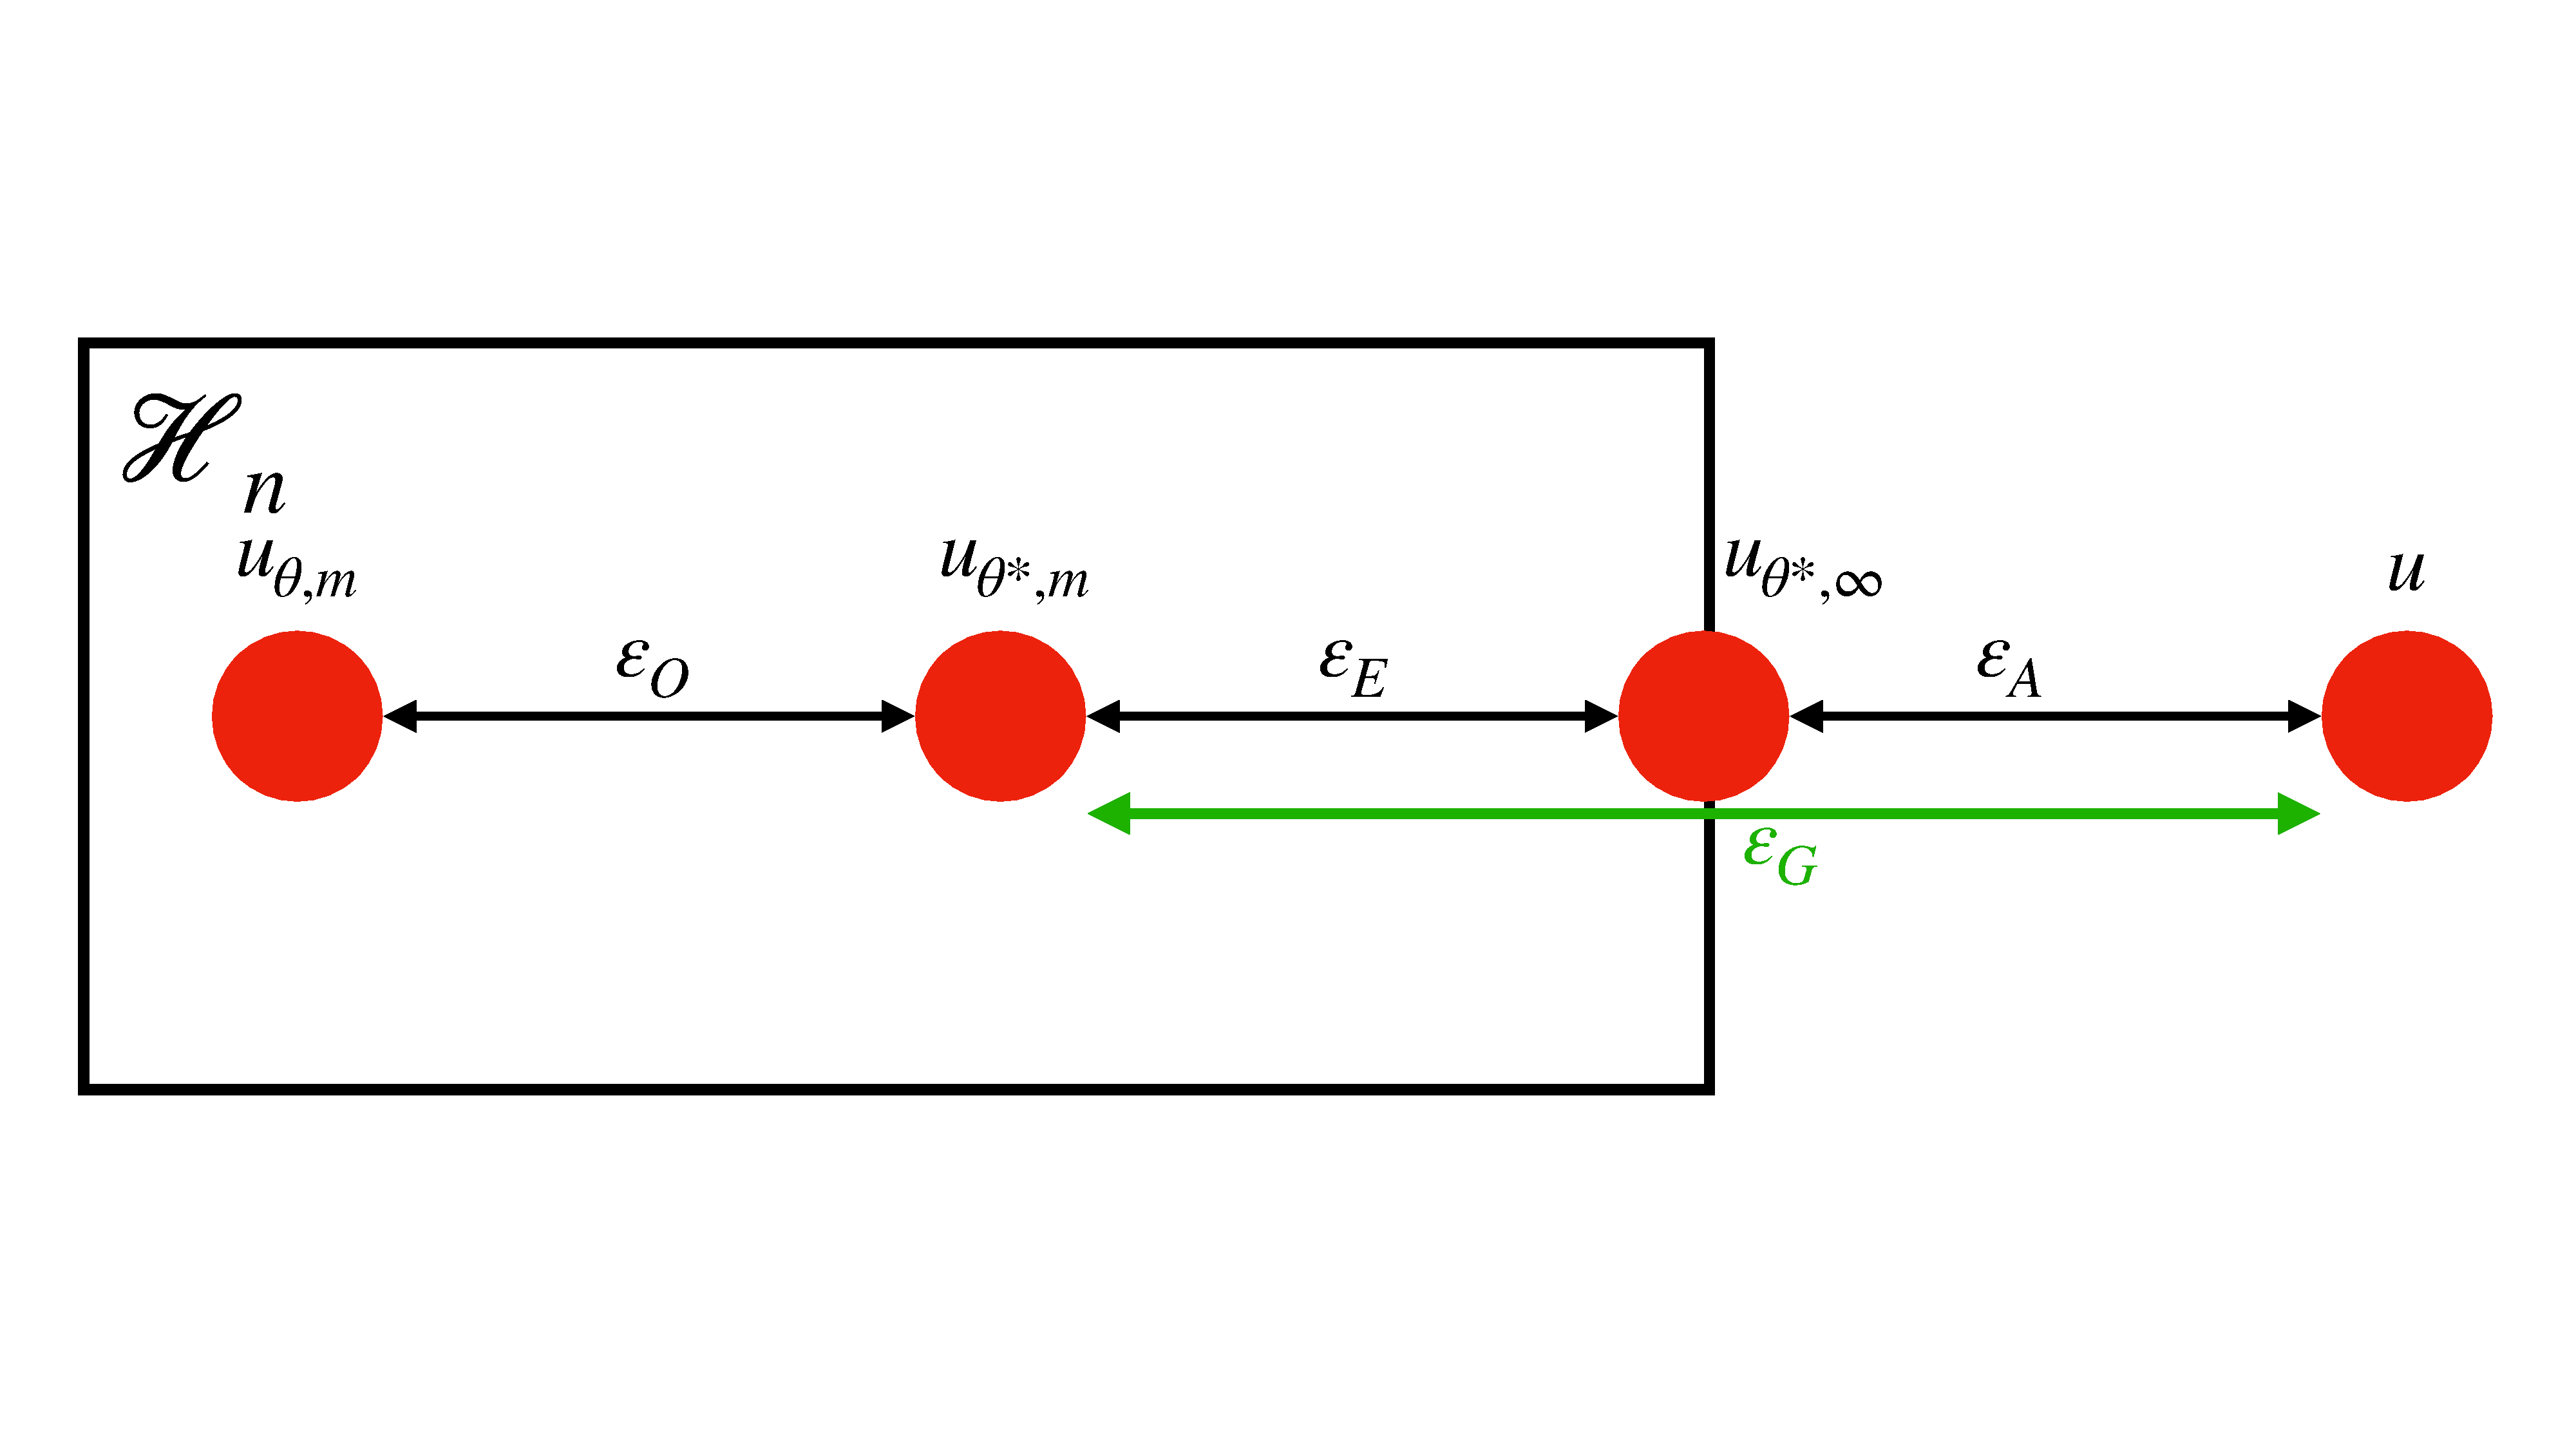
\includegraphics[width=0.9\columnwidth]{GeneralisationError.pdf}
	\caption{Illustration of the total errors. $\mathcal{H}_n$ is the chosen function class. u is the solution to the underlying PDE. The number of training data is m. $u_{\theta^*,m}$ is a minimiser of the loss with m data. $u_{\theta^*,\infty}$ is a function in $\mathcal{H}_n$ that minimises the loss with infinitely many data. $u_{\theta,m}$ is the approximation that one obtains in practice.}
	\label{fig:generalisation_error}
\end{figure}

However, these estimates do not show that a practical optimiser will achieve a sufficiently small training loss. Let $\Theta_N$ denote the parameter space for networks of width $N$. The optimisation error is $|\mathcal{L}(\widehat{\theta})-\inf_{\theta\in\Theta_N}\mathcal{L}(\theta)|$, where $\widehat{\theta}$ denotes the parameters returned by the optimiser. Existing results either study exact or approximate minimisers, or give conditional estimates in terms of the loss achieved after training. Recent analyses provide training improvements in neural-tangent-kernel or random-feature regimes \cite{ZhaoLuo_TrainingConvergence}, but these assumptions do not cover the finite-width free-knot parametrisation considered here.

This optimisation gap is especially relevant for the DRM. For a symmetric coercive problem, the Ritz functional is strictly convex in $u$, and its energy gap is equivalent to the squared energy norm. However, using a nonlinear map $\theta\mapsto u_\theta$ does not preserve this property when moving to parameter space. In a shallow ReLU network, fixed biases give a convex quadratic problem in the weights, while joint weight-bias training produces a non-convex free-knot problem.

Our aim is therefore not to prove convergence for general PINNs or deep networks. We instead identify cases where convergence can be observed by isolating these mechanisms for shallow ReLU-type networks, where biases admit an explicit interpretation as knot locations. This structure permits separate treatment of conditioning, coefficient optimisation and knot placement.

\subsection{Related Works}

Empirical studies have shown that the expressivity of a neural network does not guarantee that a PINN can be trained accurately. Krishnapriyan et al.\ \cite{Krishnapriyan_PINNFailure} consider equations containing convection, reaction and diffusion terms. They show that standard PINNs can fail even when the network is sufficiently expressive. This failure is instead linked to the conditioning and optimisation of the PDE-based loss function.

Grossmann et al.\ \cite{Grossmann_PINNFEM} provide a direct comparison between PINNs and the Finite Element Method (FEM). They consider Poisson problems in one, two and three dimensions, together with the Allen--Cahn and semilinear Schr\"odinger equations. Across their test problems, PINNs do not outperform FEM when solution time and accuracy are considered together. FEM is often both faster and more accurate, although the trained PINNs can be cheaper to evaluate at new points. These experiments do not prove that FEM must always outperform PINNs. They do, however, show that the expected expressivity of a network is not reliably realised through standard training.

The comparison by Grossmann et al.\ does not include the DRM. It should therefore not be treated as direct evidence of DRM failure. However, the DRM inherits the same parameter-space optimisation problem. Further difficulties can also arise through the enforcement of boundary conditions. For example, Courte and Zeinhofer \cite{CourteZeinhofer_RobinPretraining} show that the naive penalty formulation becomes unstable as the boundary penalty is increased.

The question considered here is narrower than the generalisation problem. Let $\Theta_N$ denote the parameter space of the chosen network and define
\begin{equation*}
    \theta^\star = \argmin_{\theta\in\Theta_N} \mathcal{L}(\theta).
\end{equation*}
Given parameters $\widehat{\theta}$ returned by training, the optimisation error is
\begin{equation*}
    \mathcal{L}(\widehat{\theta})-\mathcal{L}(\theta^\star).
\end{equation*}
Our aim is to understand how this error can be controlled. Approximation and quadrature errors remain separate parts of the full convergence problem.

The parameter space non-convexity in arises from the composition of the loss functional with the neural network. In general, the loss has the form
\begin{equation*}
    \mathcal{L}(\theta)=\mathcal{F}(u_\theta),
\end{equation*}
where $\mathcal{F}$ is a residual or energy functional. Even when $\mathcal{F}$ is convex as a function of $u$, the map $\theta\mapsto u_\theta$ is nonlinear and non-unique. Hence, $\theta\mapsto\mathcal{L}(\theta)$ need not be convex. Permutations and rescalings of the network parameters can also represent the same function, producing further degeneracy in the loss landscape.

The choice of optimiser determines how this landscape is traversed. Common optimisers use local derivative information and provide no general mechanism for identifying the basin containing a global minimiser. This does not mean that an optimiser remains inside a fixed basin: momentum, stochastic gradients and line searches can move the parameters between different regions. However, none of these mechanisms guarantees that a favourable basin will be found.

Adam \cite{KingmaBa_Adam} is a first-order method which rescales the gradient using estimates of its first and second moments. Its low per-iteration cost and tolerance of noisy gradients make it useful during the early stages of training. It is therefore often interpreted as providing an exploratory stage. This interpretation is empirical rather than a general property of the method.

Quasi-Newton methods such as BFGS and L-BFGS instead build an approximation to the inverse Hessian from previous gradients. They are more expensive per iteration but can give faster local convergence once training has reached a suitable region. Rathore et al.\ \cite{Rathore_PINNLossLandscape} relate poor PINN training to ill-conditioning induced by the differential operator. Their experiments show that Adam followed by L-BFGS is more effective than either method used separately. Here, Adam provides an initial training stage, while L-BFGS gives a more accurate local refinement.

More recent work has considered self-scaled BFGS and Broyden methods. Kiyani et al.\ \cite{Kiyani_OptimizingOptimizer} report substantial improvements from self-scaled Broyden methods across several PINN benchmarks. Energy natural gradient descent provides a related approach based on the geometry of the loss functional \cite{MullerZeinhofer_ENGD}. Its function-space update corresponds to a Newton direction projected onto the tangent space of the network. These methods can reduce the loss more efficiently within a suitable region, but they do not provide a general method for locating the global minimiser. Their reported advantages are also empirical and problem-dependent.

A different approach is to alter the structure of the optimisation problem. Appella et al.\ \cite{AppellaEtAl} consider univariate function approximation using shallow ReLU networks and Free Knot Splines (FKS). After collecting the affine terms, a shallow ReLU network can be written as
\begin{equation*}
    u_{\theta}(x)
    =
    c_0+c_1x+\sum_{i=1}^{N}a_i(x-k_i)_+,
\end{equation*}
where the breakpoints $k_i$ are determined by the inner weights and biases. A piecewise linear FKS can instead be written as
\begin{equation*}
    u_{\mathrm{FKS}}(x)
    =
    \sum_{i=0}^{N-1}w_i\phi_i(x),
\end{equation*}
where $\phi_i$ are local hat functions associated with the knots $k_i$. These representations span the same space of continuous piecewise linear functions. They therefore have the same theoretical expressivity.

The two representations have very different conditioning. The ReLU basis functions have non-local support, whereas each FKS basis function is supported only on neighbouring cells. For uniformly distributed knots, Appella et al.\ show that the normal equations for the FKS weights have condition number $\mathcal{O}(1)$. The corresponding ReLU problem has condition number $\mathcal{O}(N^4)$. Thus, two equivalent representations can produce very different training behaviour.

Appella et al.\ separate the problem of finding the knots from that of finding the weights. The knot locations are first estimated using an interpolating FKS. Let
\begin{equation*}
    h_i=k_{i+1}-k_i
\end{equation*}
denote the length of the $i$th cell. The leading contribution to the squared interpolation error on this cell is
\begin{equation*}
    \int_{k_i}^{k_{i+1}}
    \left(u-\Pi_1u\right)^2\,dx
    \approx
    \frac{1}{120}h_i^5
    \left|u''(k_{i+1/2})\right|^2.
\end{equation*}
The error is balanced between cells by imposing
\begin{equation*}
    h_i\left|u''(k_{i+1/2})\right|^{2/5}
    =
    \text{constant}.
\end{equation*}
This is the equidistribution condition. It concentrates knots in regions of high curvature, where a piecewise linear approximation requires greater resolution.

In the continuous limit, the knots are generated through a map $x=x(\xi)$ from a uniform computational coordinate $\xi\in[0,1]$. The equidistribution condition becomes
\begin{equation*}
    \frac{dx}{d\xi}
    \left|u''(x(\xi))\right|^{2/5}
    =
    \text{constant}.
\end{equation*}
The knots are then given by $k_i=x(i/(N-1))$. Alternatively, the same condition can be enforced through an equidistribution-based loss. Under suitable regularity assumptions, the resulting interpolating FKS has squared $L^2$ error of order $\mathcal{O}(N^{-4})$.

Once the knots have been located, the FKS weights are found through a well-conditioned linear least-squares problem. The FKS weights can then be mapped to the coefficients of the equivalent ReLU network using a tridiagonal linear transformation. This acts as a preconditioner for the ReLU representation. Appella et al.\ show that this two-level procedure recovers accurate approximations for regular, singular and rapidly varying target functions where direct ReLU training performs poorly.

A limitation of this method is that the target function $u$ and its curvature are assumed to be available. This is reasonable for a supervised approximation problem, but not when $u$ is the unknown solution of a differential equation. In the latter case, the monitor function must be estimated from the current approximation or inferred from the PDE. The stability of repeatedly updating this estimate must also be considered.

The FKS representation gives a direct relation to FEM. Once the knots are fixed, the functions $\phi_i$ are precisely the one-dimensional piecewise linear finite element basis functions. For a linear coercive problem, substituting
\begin{equation*}
    u_h(x)=\sum_{i=0}^{N-1}w_i\phi_i(x)
\end{equation*}
into the Ritz energy produces a sparse linear system for the weights,
\begin{equation*}
    A\mathbf{w}=\mathbf{f}.
\end{equation*}
The nonlinear part of the problem is therefore moved into the selection of the knot locations. The weights are then calculated using the same type of linear solve used within FEM.

This does not imply a general equivalence between neural networks and FEM. The correspondence is exact for shallow univariate ReLU networks, while deeper networks and higher-dimensional problems have a more complicated structure. Nevertheless, it shows that part of the neural-network training problem can be reinterpreted as an adaptive finite element problem. The present work builds on this observation by separating the placement of the knots from the solution of the DRM weight problem.

\subsection{Contributions}

The approach taken in this paper is deliberately restrictive. We begin with standard PINN and DRM training and identify which parts of the method prevent reliable convergence. The problem is then simplified until these parts can be treated independently. Our contribution is therefore not another choice of optimiser or network architecture. Instead, we identify a setting in which the optimisation problem can be related directly to classical approximation theory.

Our first contribution is an investigation of several common explanations for training failure. Increasing the number of collocation or quadrature points can improve the approximation of the continuous loss. However, it does not remove the non-convexity of the parameter-space problem. In this setting, there is therefore no monotonic relation between the number of points and the error produced after training. 

The optimiser and preconditioner have a similarly limited role. They can improve the conditioning and local rate of convergence, but do not provide a general mechanism for locating a global minimiser. Changes to the activation function and network architecture can alter both the approximation space and the loss landscape. However, these choices do not remove the underlying difficulty of jointly optimising all network parameters. 

The main structural observation is that the weights and biases of a shallow ReLU network play different mathematical roles. After normalisation, the network can be written in the form
\begin{equation*}
    u_{\mathbf{w},\mathbf{k}}(x)
    =
    w_0+w_1x+\sum_{i=1}^{N}w_{i+1}(x-k_i)_+,
\end{equation*}

where the weights $\mathbf{w}$ act as basis coefficients and the biases determine the knot locations $\mathbf{k}$. Joint training couples these two roles. This introduces a free-knot optimisation problem in which knots can move, collide or leave the domain.

For fixed knots, the network is linear in its weights. In the case of a linear coercive Ritz problem, the discrete energy takes the form
\begin{equation*}
    \mathcal{E}_h(\mathbf{w};\mathbf{k})
    =
    \frac{1}{2}\mathbf{w}^{T}A(\mathbf{k})\mathbf{w}
    -
    \mathbf{f}(\mathbf{k})^{T}\mathbf{w}.
\end{equation*}
Provided that the basis is independent and the quadrature rule preserves coercivity, $A(\mathbf{k})$ is positive definite. The weight problem is therefore strictly convex and has a unique minimiser. Gradient descent converges to this minimiser when the step size is chosen appropriately. Equivalently, the weights can be calculated by solving
\begin{equation*}
    A(\mathbf{k})\mathbf{w}=\mathbf{f}(\mathbf{k}).
\end{equation*}

Our main algorithmic contribution is to separate this convex weight problem from the nonlinear placement of the knots. The weights are first trained with the knots held fixed. The knots are then updated using an equidistribution principle, building on the FKS method of Appella et al.\ \cite{AppellaEtAl}. Given a monitor function $M$, the knot map $x=x(\xi)$ is chosen to satisfy
\begin{equation*}
    M(x(\xi))\frac{dx}{d\xi}
    =
    \text{constant}.
\end{equation*}
For piecewise linear $L^2$ approximation, the corresponding monitor is proportional to $|u''|^{2/5}$. In the PDE setting, this monitor must be estimated from the current approximation. The two steps are repeated until the weights and knot locations stabilise.

This separation gives two distinct convergence statements. For each fixed set of admissible knots, the weight optimisation converges to the unique minimiser of the discrete Ritz energy. Separately, equidistribution provides approximation estimates as the number of knots increases, subject to regularity and mesh assumptions. Together, these results give convergence when the knot sequence is suitably equidistributed and the quadrature rule resolves the resulting approximation space. They do not, without further assumptions, prove global convergence of every alternating weight--knot iteration.

The analysis is restricted to shallow networks in one spatial dimension and to problems admitting a coercive Ritz formulation. This restriction allows the biases to be interpreted explicitly as ordered knot locations. It also allows the conditioning and uniqueness of the weight problem to be analysed directly. The result should not be interpreted as a convergence theorem for general deep PINNs or DRM approximations.

Coercivity alone does not ensure that every discrete solution is non-oscillatory. In convection-dominated problems, the approximation can exhibit oscillations similar to those produced by an unstable Galerkin finite element method. This occurs when the knot spacing does not resolve the small diffusive scale. The limitation is therefore associated with the discrete approximation space and not only with the optimiser. Suitable refinement or stabilisation remains necessary in this regime.

Finally, the split representation gives a direct connection to FEM. With fixed knots, the associated FKS basis is the standard one-dimensional piecewise linear finite element basis. Minimising the DRM energy over the weights is then equivalent to solving the corresponding finite element linear system. Using gradient descent does not change this underlying problem; it replaces the direct linear solve with an iterative optimisation procedure. The authors identify this formulation as a potential starting point for analysing whether similar structures persist in deep neural networks.

The nonlinear part of the method is consequently moved into the placement of the knots. In this setting, the network can be interpreted as an adaptive finite element approximation written in neural-network parameters. This provides a framework in which PINN or DRM training can be compared directly with FEM, complementing the empirical comparison of Grossmann et al.\ \cite{Grossmann_PINNFEM}. It also identifies which apparent differences arise from the approximation space and which arise only from the training procedure.


\section{Shallow Deep Ritz Method}

\subsection{Toy Problem and Ritz Formulation}
\label{sec:EllipticProblem}

We consider the singularly perturbed reaction--diffusion problem
\begin{equation}
    -\varepsilon^2 u''(x)+u(x)=1,
    \qquad x\in(0,1),
    \label{eq:toy_problem}
\end{equation}
subject to
\begin{equation*}
    u(0)=u(1)=0,
\end{equation*}
where \(0<\varepsilon\leq 1\). Define the differential operator
\begin{equation*}
    \mathcal A_\varepsilon v
    =
    -\varepsilon^2v''+v.
\end{equation*}
For each fixed \(\varepsilon>0\), this is a linear elliptic problem with the exact solution
\begin{equation}
    u(x)
    =
    1-
    \frac{\cosh\left((x-\frac12)/\varepsilon\right)}
         {\cosh\left(1/(2\varepsilon)\right)}.
    \label{eq:toy_exact_solution}
\end{equation}
The solution satisfies \(0\leq u\leq1\). As \(\varepsilon\) decreases, it approaches \(1\) in the interior and develops boundary layers of width \(O(\varepsilon)\) near \(x=0\) and \(x=1\). This provides a simple problem in which the required spatial resolution is known explicitly.

The Green's function associated with \(\mathcal A_\varepsilon\) and the homogeneous boundary conditions is
\begin{equation}
    G_\varepsilon(x,s)
    =
    \frac{
        \sinh\left(x_{<}/\varepsilon\right)
        \sinh\left((1-x_{>})/\varepsilon\right)
    }{
        \varepsilon\sinh(1/\varepsilon)
    },
    \label{eq:toy_green_function}
\end{equation}
where
\begin{equation*}
    x_{<}=\min\{x,s\},
    \qquad
    x_{>}=\max\{x,s\}.
\end{equation*}
The solution can therefore be written as
\begin{equation*}
    u(x)=\int_0^1G_\varepsilon(x,s)\,ds.
\end{equation*}

Let \(v\) satisfy the boundary conditions and define its residual by
\begin{equation*}
    r_v=\mathcal A_\varepsilon v-1.
\end{equation*}
The error satisfies
\begin{equation}
    v(x)-u(x)
    =
    \int_0^1G_\varepsilon(x,s)r_v(s)\,ds.
    \label{eq:green_error_representation}
\end{equation}
Since \(G_\varepsilon\geq0\) and
\begin{equation*}
    \int_0^1G_\varepsilon(x,s)\,ds
    =
    u(x)\leq1,
\end{equation*}
it follows that
\begin{equation}
    \|v-u\|_{L^\infty(0,1)}
    \leq
    \|r_v\|_{L^\infty(0,1)}.
    \label{eq:continuous_residual_stability}
\end{equation}
Thus, control of the residual throughout the domain gives direct control of the solution error.

This estimate also illustrates the stability requirement in a classical collocation method. Let \(V_h^{\mathrm{col}}\) be a smooth finite-dimensional trial space satisfying the homogeneous boundary conditions. Given collocation points
\begin{equation*}
    X_h=\{x_i\}_{i=1}^{M}\subset(0,1),
\end{equation*}
the collocation approximation \(u_h^{\mathrm{col}}\in V_h^{\mathrm{col}}\) is defined by
\begin{equation}
    \mathcal A_\varepsilon u_h^{\mathrm{col}}(x_i)=1,
    \qquad i=1,\ldots,M.
    \label{eq:classical_collocation}
\end{equation}
The point values in \eqref{eq:classical_collocation} must control the trial function between the collocation points. A suitable discrete stability condition is
\begin{equation}
    \|v_h\|_{L^\infty(0,1)}
    \leq
    C_{\mathrm{col}}
    \max_{1\leq i\leq M}
    |\mathcal A_\varepsilon v_h(x_i)|,
    \qquad
    v_h\in V_h^{\mathrm{col}}.
    \label{eq:collocation_stability}
\end{equation}
This requires the collocation equations to be uniquely solvable. For convergence, \(C_{\mathrm{col}}\) must also remain controlled as the trial space is refinedn.

For any \(w_h\in V_h^{\mathrm{col}}\), equations
\eqref{eq:classical_collocation} and \eqref{eq:collocation_stability} give
\begin{equation*}
    \|u_h^{\mathrm{col}}-w_h\|_{L^\infty}
    \leq
    C_{\mathrm{col}}
    \max_i
    |\mathcal A_\varepsilon(u-w_h)(x_i)|.
\end{equation*}
Consequently,
\begin{equation}
    \|u-u_h^{\mathrm{col}}\|_{L^\infty}
    \leq
    \inf_{w_h\in V_h^{\mathrm{col}}}
    \left\{
        \|u-w_h\|_{L^\infty}
        +
        C_{\mathrm{col}}
        \max_i
        |\mathcal A_\varepsilon(u-w_h)(x_i)|
    \right\}.
    \label{eq:collocation_error_estimate}
\end{equation}
Convergence therefore requires both approximation and discrete stability.

The locations of the points enter through \(C_{\mathrm{col}}\). They also determine the fill distance
\begin{equation*}
    h_{X}
    =
    \sup_{x\in[0,1]}
    \min_{x_i\in X_h}|x-x_i|.
\end{equation*}
For any continuously differentiable residual,
\begin{equation*}
    \|r_v\|_{L^\infty}
    \leq
    \max_i|r_v(x_i)|
    +
    h_X\|r_v'\|_{L^\infty}.
\end{equation*}
Hence, even an exact zero residual at every collocation point does not control the continuous residual unless \(h_X\) and the variation of \(r_v\) are also controlled. Increasing the number of points need not reduce \(h_X\) if the new points remain concentrated in an already resolved region. For \eqref{eq:toy_problem}, the point set must also resolve the \(O(\varepsilon)\) boundary layers.

We now introduce the variational formulation used by the DRM. Let
\begin{equation*}
    V=H_0^1(0,1)
\end{equation*}
and define
\begin{align}
    a_\varepsilon(w,v)
    &=
    \int_0^1
    \left(
        \varepsilon^2w'v'+wv
    \right)\,dx,
    \\
    \ell(v)
    &=
    \int_0^1v\,dx.
\end{align}
The weak problem is to find \(u\in V\) such that
\begin{equation}
    a_\varepsilon(u,v)=\ell(v),
    \qquad
    v\in V.
    \label{eq:toy_weak_form}
\end{equation}
The bilinear form is continuous. For each fixed \(\varepsilon>0\), it is also coercive since
\begin{equation*}
    a_\varepsilon(v,v)
    =
    \varepsilon^2\|v'\|_{L^2}^2
    +
    \|v\|_{L^2}^2
    \geq
    \min\{\varepsilon^2,1\}
    \|v\|_{H^1}^2.
\end{equation*}
The Lax--Milgram theorem therefore gives a unique weak solution. We define the associated energy norm by
\begin{equation}
    \|v\|_\varepsilon^2
    =
    a_\varepsilon(v,v)
    =
    \varepsilon^2\|v'\|_{L^2}^2
    +
    \|v\|_{L^2}^2.
    \label{eq:energy_norm}
\end{equation}
The coercivity constant in the standard \(H^1\) norm deteriorates as \(\varepsilon\to0\). The energy norm retains the natural scaling of the problem.

The corresponding Ritz functional is
\begin{equation}
    E(v)
    =
    \frac12a_\varepsilon(v,v)-\ell(v)
    =
    \frac12
    \int_0^1
    \left(
        \varepsilon^2|v'|^2+|v|^2
    \right)\,dx
    -
    \int_0^1v\,dx.
    \label{eq:toy_ritz_energy}
\end{equation}
Its unique minimiser over \(V\) is the weak solution of
\eqref{eq:toy_problem}. Moreover,
\begin{equation}
    E(v)-E(u)
    =
    \frac12a_\varepsilon(v-u,v-u)
    =
    \frac12\|v-u\|_\varepsilon^2.
    \label{eq:ritz_energy_gap}
\end{equation}
The continuous energy gap is therefore exactly equivalent to the squared solution error in the energy norm.

For a fixed finite-dimensional space \(V_h\subset V\), let
\begin{equation*}
    u_h=\arg\min_{v_h\in V_h}E(v_h).
\end{equation*}
Galerkin orthogonality gives
\begin{equation}
    \|u-u_h\|_\varepsilon
    =
    \inf_{v_h\in V_h}
    \|u-v_h\|_\varepsilon.
    \label{eq:ritz_best_approximation}
\end{equation}
Thus, when the continuous energy is minimised exactly, the error is determined entirely by the approximation properties of \(V_h\).

\subsection{Shallow Network Representation}

The notation in this section follows Appella et al.~\cite{AppellaEtAl}. Their analysis relates shallow univariate ReLU networks to Free Knot Splines (FKS). In particular, they interpret the transformed biases as knot locations and identify a linear map between the ReLU and FKS coefficient systems. We adapt this representation to the homogeneous Dirichlet problem considered here.

Let
\begin{equation*}
    \sigma(x)=(x)_+=\max\{x,0\}
\end{equation*}
denote the ReLU activation function. After choosing a common orientation for the ReLU functions, positive homogeneity gives
\begin{equation*}
    \sigma(a_i x+b_i)
    =
    a_i\sigma(x-k_i),
    \qquad
    k_i=-\frac{b_i}{a_i}.
\end{equation*}
The inner weight can therefore be absorbed into the outer coefficient. The transformed bias \(k_i\) is the breakpoint of the corresponding ReLU function. We refer to these breakpoints as knots.

After collecting the affine terms, a shallow network with \(N\) hidden units can be written as
\begin{equation}
    \widetilde u_{\mathbf c,\mathbf k}(x)
    =
    c_0+c_1x+
    \sum_{i=1}^N c_i(x-k_i)_+.
    \label{eq:shallow_relu}
\end{equation}
We assume that the knots remain within the domain and are ordered such that
\begin{equation}
    0=k_0<k_1<\cdots<k_N<k_{N+1}=1.
    \label{eq:admissible_knots}
\end{equation}
This excludes inactive knots, repeated knots and changes in their ordering.

The boundary conditions are imposed exactly. Evaluating
\eqref{eq:shallow_relu} at \(x=0\) and \(x=1\) gives
\begin{equation*}
    c_0=0,
    \qquad
    c_1=-\sum_{i=1}^N c_i(1-k_i),
\end{equation*}
where the second \(c_1\) denotes the coefficient of the affine term in
\eqref{eq:shallow_relu}. To avoid this overlap in notation, we collect the constraints and write the boundary-constrained network directly as
\begin{equation}
    u_{\mathbf c,\mathbf k}(x)
    =
    \sum_{i=1}^N
    c_i\left[
        (x-k_i)_+-(1-k_i)x
    \right].
    \label{eq:boundary_constrained_relu}
\end{equation}
Thus, \(u_{\mathbf c,\mathbf k}\in H_0^1(0,1)\) for every admissible set of knots.

For the same knot sequence, define
\begin{equation*}
    h_i=k_{i+1}-k_i,
    \qquad i=0,\ldots,N,
\end{equation*}
and let \(\phi_i\) denote the local hat function
\begin{equation}
    \phi_i(x)
    =
    \begin{cases}
        \dfrac{x-k_{i-1}}{h_{i-1}},
        &x\in[k_{i-1},k_i],\\[1.2ex]
        \dfrac{k_{i+1}-x}{h_i},
        &x\in[k_i,k_{i+1}],\\[1.2ex]
        0,
        &\text{otherwise},
    \end{cases}
    \qquad i=1,\ldots,N.
    \label{eq:hat_basis}
\end{equation}
The corresponding FKS representation is
\begin{equation}
    u_{\mathbf w,\mathbf k}(x)
    =
    \sum_{i=1}^Nw_i\phi_i(x).
    \label{eq:fks_representation}
\end{equation}
Here, \(w_i=u_{\mathbf w,\mathbf k}(k_i)\) is the value of the approximation at the \(i\)th knot.

The ReLU and FKS representations span the same space of continuous piecewise linear functions. Their coefficients have different meanings. The FKS coefficients are nodal values, while the ReLU coefficients describe changes in gradient. Setting \(w_0=w_{N+1}=0\), they satisfy
\begin{equation}
    c_i
    =
    \frac{w_{i+1}-w_i}{h_i}
    -
    \frac{w_i-w_{i-1}}{h_{i-1}},
    \qquad i=1,\ldots,N.
    \label{eq:relu_fks_transformation}
\end{equation}
Writing this relation in matrix form gives
\begin{equation*}
    \mathbf c
    =
    T(\mathbf k)\mathbf w.
\end{equation*}
For fixed knots, \(T(\mathbf k)\) is a tridiagonal linear map. Appella et al. interpret this change of coefficients as a preconditioner. Optimisation over the coefficients of the non-local ReLU basis is replaced by optimisation over the coefficients of the local FKS basis.

This change of basis can have a substantial effect on conditioning. For uniformly distributed fixed knots in the \(L^2\) approximation problem, Appella et al. show that the normal equations for the FKS coefficients have condition number \(O(1)\). The corresponding ReLU system has condition number \(O(N^4)\). The two representations therefore have the same expressivity but can give very different optimisation problems.

These estimates do not transfer directly to the DRM. Its Hessian is determined by the PDE bilinear form rather than the \(L^2\) inner product. The conditioning can therefore depend on both \(\varepsilon\) and the knot spacing. Nevertheless, the result motivates the use of the FKS parametrisation as a preconditioned representation of the shallow ReLU network.

With the fixed knots, define
\begin{equation}
    V_h(\mathbf k)
    =
    \operatorname{span}\{\phi_1,\ldots,\phi_N\}.
    \label{eq:fixed_knot_space}
\end{equation}
This is a linear approximation space. Allowing the knots to vary instead gives the nonlinear class
\begin{equation*}
    \mathcal V_N
    =
    \bigcup_{\mathbf k\in\mathcal K_N}
    V_h(\mathbf k),
\end{equation*}
where \(\mathcal K_N\) denotes the set of ordered admissible knots. The nonlinearity therefore enters through the placement of the knots.

The functions \(\phi_i\) are precisely the standard one-dimensional piecewise linear finite element basis functions. When the Ritz functional is integrated exactly, minimising it over \(V_h(\mathbf k)\) gives
\begin{equation}
    A(\mathbf k)\mathbf w
    =
    \mathbf f(\mathbf k),
    \label{eq:fem_system}
\end{equation}
where
\begin{equation*}
    A_{ij}(\mathbf k)
    =
    a_\varepsilon(\phi_j,\phi_i),
    \qquad
    f_i(\mathbf k)
    =
    \ell(\phi_i).
\end{equation*}
The shallow DRM and the corresponding \(P_1\) finite element method therefore use the same trial space and produce the same linear system. The distinction lies in how the knots are selected and how the coefficient problem is solved.


\subsection{Why Standard Training Fails}

Failure of standard training is often attributed to a single component of the method with common explanations including the optimiser, choice of activation function, network architecture, and number/placement of collocation or quadrature points. Methods addressing these issues can improve training, but do not by themselves guarantee convergence.

\

Ill-conditioning can make the optimal network parameters difficult to obtain, even when the approximation space contains an accurate solution. Appella et al.~\cite{AppellaEtAl} demonstrate this distinction for shallow ReLU networks and their equivalent free-knot spline (FKS) representation: the two representations have the same expressivity, but substantially different conditioning. Figure~\ref{fig:elliptic-parameterisation} illustrates the practical effect for the reaction--diffusion problem. The ReLU approximations remain inaccurate with both fixed and jointly trained knots. The linear hat-function basis improves the approximations, with the closest agreement obtained using trainable knots. This comparison illustrates the importance of the coefficient parameterisation, rather than expressivity alone.

\begin{figure}[htbp]
    \centering

    \begin{subfigure}[t]{0.48\textwidth}
        \centering
        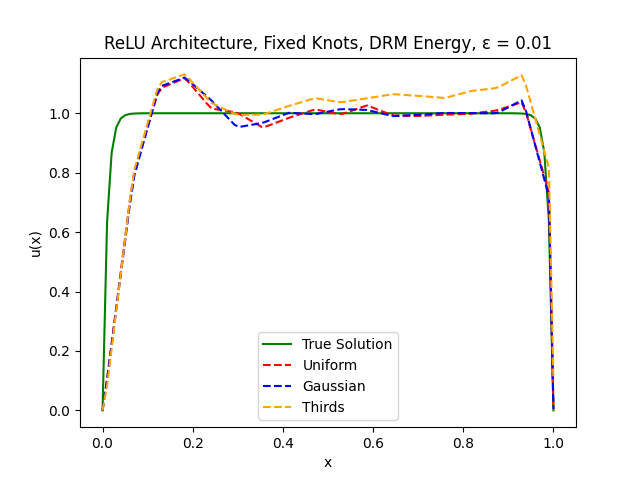
\includegraphics[width=\linewidth]{FixedKnot_ReLU_DRM.png}
        \caption{ReLU basis with fixed knots.}
        \label{fig:fixed_relu}
    \end{subfigure}
    \hfill
    \begin{subfigure}[t]{0.48\textwidth}
        \centering
        \includegraphics[width=\linewidth]
        {FreeKnot_RelU_DRM.png}
        \caption{ReLU basis with jointly trained knots.}
        \label{fig:free_relu}
    \end{subfigure}

    \medskip

    \begin{subfigure}[t]{0.48\textwidth}
        \centering
        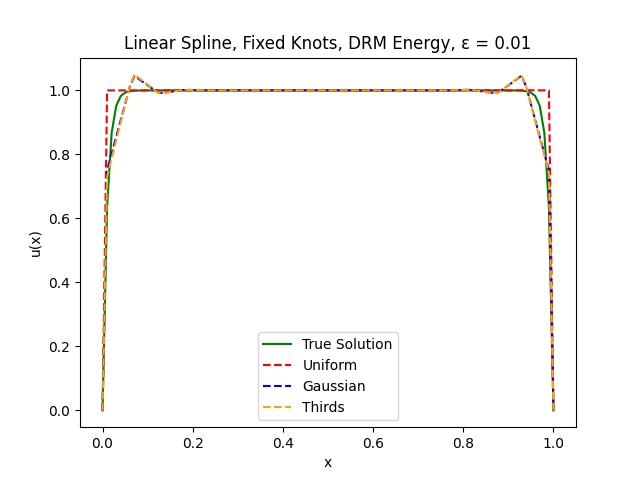
\includegraphics[width=\linewidth]
        {FixedKnot_LinearSpline_DRM.png}
        \caption{FKS basis with fixed knots.}
        \label{fig:fixed_fks}
    \end{subfigure}
    \hfill
    \begin{subfigure}[t]{0.48\textwidth}
        \centering
        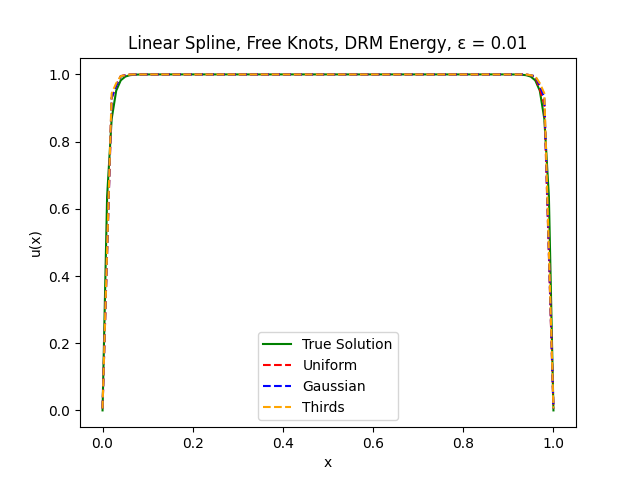
\includegraphics[width=\linewidth]
        {FreeKnot_LinearSpline_DRM.png}
        \caption{FKS basis with jointly trained knots.}
        \label{fig:free_fks}
    \end{subfigure}

    \caption{
        Effect of the coefficient parametrisation and knot training
        for the reaction--diffusion problem with
        \(\varepsilon=0.01\).
        The ReLU and FKS bases span the same piecewise linear
        approximation space. Direct training in the ReLU basis is
        inaccurate, while the FKS parametrisation gives accurate
        approximations with both fixed and trainable knots.
    }
    \label{fig:relu_fks_comparison}
\end{figure}

However, conditioning also depends on the differential operator and the loss. For the convection--diffusion problem, the integrating-factor energy introduces the weight $e^{-x/\varepsilon}$, producing large differences in the contribution of errors across the domain. Figure~\ref{fig:convection-training} shows that the FKS representation with jointly trained knots remains inaccurate for this problem, despite its success in Figure~\ref{fig:elliptic-parameterisation}. Energy natural gradient methods address the interaction between the objective and its parameterisation through a metric induced by the function-space Hessian~\cite{MullerZeinhofer_ENGD}. Related approaches address unequal learning rates: NTK-based loss weighting balances different loss components~\cite{wang2022ntk}, while Fourier-feature embeddings can alleviate spectral bias in multiscale problems~\cite{wang2021eigenvector}.

\begin{figure}
    \centering
    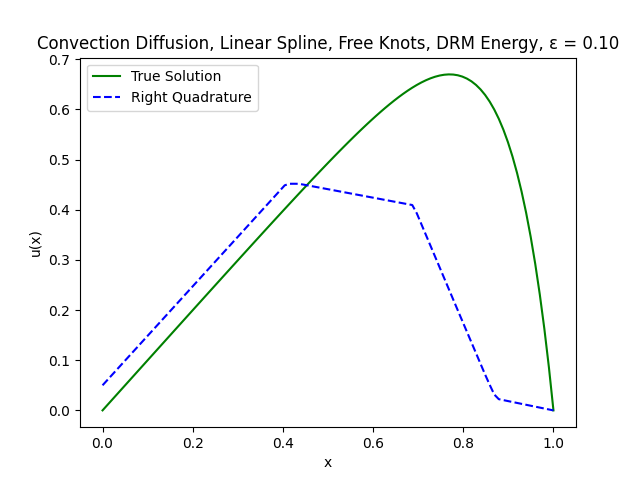
\includegraphics[width=0.5\linewidth]{DRM_Failed_Split.png}
    \caption{Failure of standard joint training for the convection--diffusion
    problem
    \(-\varepsilon u''+u'=1\), with
    \(u(0)=u(1)=0\) and \(\varepsilon=0.1\).
    The FKS coefficients and knots are trained simultaneously using
    the DRM energy and quadrature refined towards the outflow boundary.
    The resulting approximation remains inaccurate, showing that the
    FKS parametrisation and suitable quadrature are not sufficient for
    reliable joint training.}
    \label{fig:fks_joint_failure}
\end{figure}

These results show that improving the basis can substantially improve training without ensuring accuracy across problems. Preconditioning and changes to the representation address important obstacles, but do not generally remove non-convexity in the network parameters. The figures demonstrate the limitations of these training configurations; they do not, by themselves, establish whether the remaining errors arise from ill-conditioning, non-convexity or incomplete optimisation.

\
 
The number and distribution of collocation points determine how well the discrete residual represents the governing equation across the domain. Shin et al.~\cite{ShinDarbonKarniadakis_Convergence} establish convergence as the sample count increases for minimisers of a suitably regularised PINN loss, under assumptions on sampling, regularity and approximation. Mishra and Molinaro~\cite{MishraMolinaro_GenErr} bound the solution error using PDE stability, the achieved training error and quadrature error. These results do not imply that increasing the number of points alone guarantees an accurate trained network: the optimisation error must also be controlled. Similarly, in DRM, refining the quadrature improves the approximation of the energy but does not ensure its minimisation. Nonuniform sampling also requires appropriate weights when approximating a specified domain integral.

Figure~\ref{fig:collocation-count-study} illustrates this distinction for the reaction--diffusion problem with $\varepsilon=0.01$. We use $N=30,90,300,900$ collocation points, allocating one third uniformly within each of $[0,\varepsilon]$, $[\varepsilon,1-\varepsilon]$ and $[1-\varepsilon,1]$. Equal residual weights emphasise the boundary regions. The width-100 tanh network, initial parameters and training budget of $20{,}000$ Adam steps are held fixed. Despite this thirtyfold increase in sampling, the approximations remain similar and inaccurate, with $L^2$ errors between $0.155$ and $0.161$. Thus, additional points alone do not resolve the training failure in this experiment. This observation does not contradict convergence results for loss minimisers, nor establish non-convexity as the cause of the remaining error.

\begin{figure}[htbp]
    \centering
    \begin{subfigure}[c]{0.49\textwidth}
        \vspace{0pt}
        \centering
        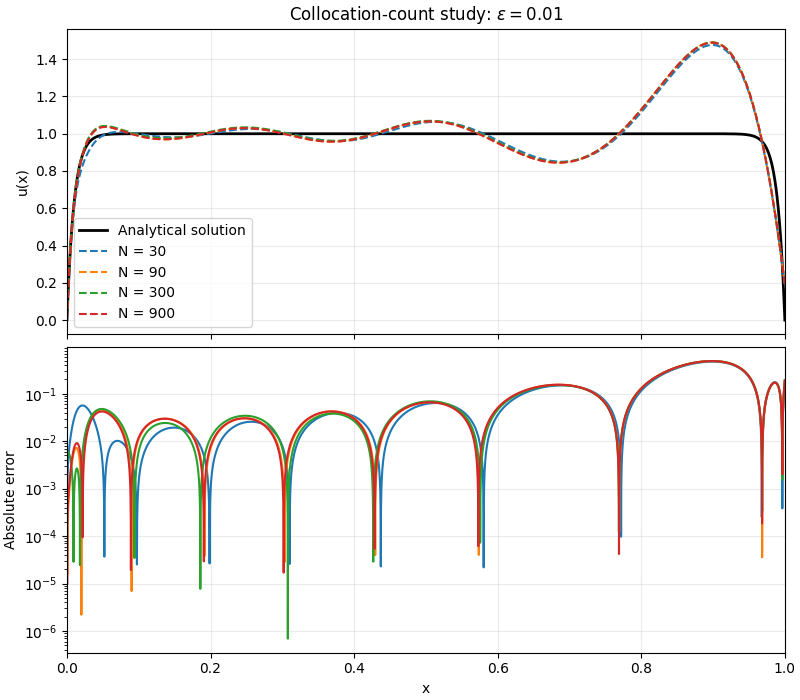
\includegraphics[width=\linewidth]{collocation_comparison.png}
        \caption{Approximations and pointwise absolute errors.}
        \label{fig:collocation-comparison}
    \end{subfigure}
    \hfill
    \begin{subfigure}[c]{0.49\textwidth}
        \centering
        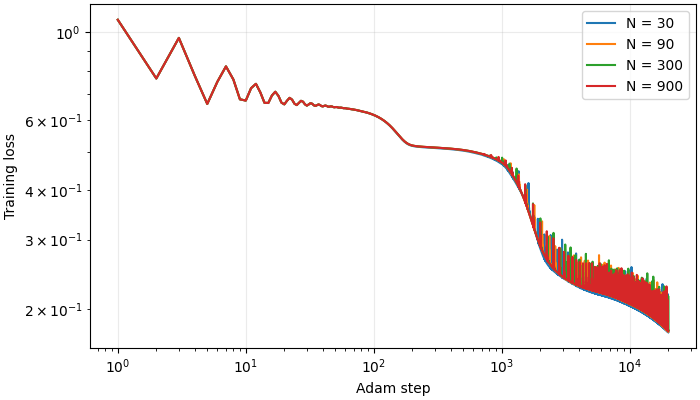
\includegraphics[width=\linewidth]{Collocation_loss.png}
        \caption{Training loss against optimiser steps.}
        \label{fig:collocation-loss}
    \end{subfigure}
    \caption{Effect of collocation-point count for $-\varepsilon^2u''+u=1$, with zero Dirichlet conditions and $\varepsilon=0.01$. One third of the points is distributed uniformly within each of $[0,\varepsilon]$, $[\varepsilon,1-\varepsilon]$ and $[1-\varepsilon,1]$. All runs use identical initial parameters and $20{,}000$ Adam steps with learning rate $0.01$.}
    \label{fig:collocation-count-study}
\end{figure}

\

Beyond the discretisation of the loss, optimisation is also affected by how the network parameters determine the approximation. The coefficients and knot locations play different roles in a shallow ReLU network: the coefficients determine the linear combination of basis functions, while the hidden-layer weights and biases determine their activation points. Joint optimisation couples these roles nonlinearly, even when the underlying energy is convex in the represented function. For fixed knots, a convex DRM energy remains convex in the spline coefficients, whereas optimisation over the knot locations is generally non-convex. Unconstrained knot motion also permits knots to approach or cross one another. Nearly coincident activation points can produce nearly dependent ReLU basis functions and worsen conditioning. Preserving knot order avoids crossings, although additional separation constraints may be needed to prevent knot coalescence.

Although these approaches provide substantial improvements over standard training, a central issue remains: they do not generally guarantee that optimisation reaches parameters yielding an accurate solution. The nonlinear parameterisation of a deep network generally produces a non-convex loss, even when the underlying energy is convex in function space. Consequently, guarantees formulated for global minimisers do not automatically apply to the parameters returned by gradient-based training. An end-to-end accuracy guarantee must also control the optimisation error, for example by establishing convergence to a global minimiser or to a sufficiently small objective gap.

One route is a suitable initialisation within a region where convergence to an accurate minimiser can be established. Such a guarantee requires local assumptions on the objective and the optimisation method; proximity alone does not imply a convex neighbourhood. Another route is to use a parameterisation for which the objective is convex, as occurs for a convex DRM energy with fixed basis functions and trainable linear coefficients. Although other guarantees are possible for structured non-convex problems, neither improved sampling nor preconditioning alone supplies the missing control of optimisation error. The following section makes use of this methodology by restricting the network architecture to a singular hidden layer.


\section{Split Deep Ritz Training}

\subsection{Fixed Knot Optimisation}

Let \(\mathbf k\in\mathcal K_N\) be any admissible knot sequence. During the coefficient step, \(\mathbf k\) is held constant and the approximation is written as
\begin{equation*}
    u_{\mathbf w,\mathbf k}(x)
    =
    \sum_{i=1}^Nw_i\phi_i(x).
\end{equation*}
The basis functions are now fixed and the map
\begin{equation*}
    \mathbf w
    \longmapsto
    u_{\mathbf w,\mathbf k}
\end{equation*}
is linear.

Let \(a_{\varepsilon,h}\) and \(\ell_h\) denote the quadrature approximations of the bilinear and linear forms introduced in Section~2.1. The discrete Ritz energy is
\begin{equation}
    E_h(\mathbf w;\mathbf k)
    =
    \frac12
    a_{\varepsilon,h}
    (u_{\mathbf w,\mathbf k},u_{\mathbf w,\mathbf k})
    -
    \ell_h(u_{\mathbf w,\mathbf k})
    =
    \frac12\mathbf w^TA(\mathbf k)\mathbf w
    -
    \mathbf f(\mathbf k)^T\mathbf w,
    \label{eq:fixed_knot_energy}
\end{equation}
where
\begin{equation*}
    A_{ij}(\mathbf k)
    =
    a_{\varepsilon,h}(\phi_j,\phi_i),
    \qquad
    f_i(\mathbf k)
    =
    \ell_h(\phi_i).
\end{equation*}

Assume that the basis functions are linearly independent and that the quadrature rule preserves coercivity on \(V_h(\mathbf k)\). Then \(A(\mathbf k)\) is symmetric positive definite. Consequently, \(E_h(\cdot;\mathbf k)\) is strictly convex and has the unique minimiser
\begin{equation}
    \mathbf w^\star(\mathbf k)
    =
    A(\mathbf k)^{-1}\mathbf f(\mathbf k).
    \label{eq:fixed_knot_minimiser}
\end{equation}
The energy gap satisfies
\begin{equation}
    E_h(\mathbf w;\mathbf k)
    -
    E_h(\mathbf w^\star;\mathbf k)
    =
    \frac12
    (\mathbf w-\mathbf w^\star)^T
    A(\mathbf k)
    (\mathbf w-\mathbf w^\star).
    \label{eq:discrete_energy_gap}
\end{equation}
Thus, convergence of the coefficient vector is equivalent to convergence in the discrete energy norm.

For example, gradient descent gives
\begin{equation}
    \mathbf w^{n+1}
    =
    \mathbf w^n
    -
    \eta
    \left(
        A(\mathbf k)\mathbf w^n-\mathbf f(\mathbf k)
    \right).
    \label{eq:fixed_knot_gradient_descent}
\end{equation}
For any initial value \(\mathbf w^0\), this iteration converges to \(\mathbf w^\star(\mathbf k)\) whenever
\begin{equation*}
    0<\eta<
    \frac{2}{\lambda_{\max}(A(\mathbf k))}.
\end{equation*}
The rate depends on the condition number of \(A(\mathbf k)\). Preconditioning changes this rate, but not the location or uniqueness of the minimiser.

When the Ritz functional is integrated exactly, \(A(\mathbf k)\) and \(\mathbf f(\mathbf k)\) are precisely the stiffness matrix and load vector of the \(P_1\) finite element method on the mesh \(\mathbf k\). The resulting approximation therefore satisfies
\begin{equation*}
    \|u-u_{\mathbf w^\star,\mathbf k}\|_\varepsilon
    =
    \inf_{v_h\in V_h(\mathbf k)}
    \|u-v_h\|_\varepsilon.
\end{equation*}
With numerical quadrature, an additional consistency error remains.

The coefficient step is therefore not a non-convex neural-network problem. It is a finite element linear system written as an optimisation problem. Replacing the linear solve by gradient descent does not change the underlying discrete problem and will usually be less efficient than a sparse direct solver. Its importance here is that convergence of this part of the training procedure can be guaranteed.

This result does not yet guarantee convergence to the exact PDE solution. The approximation error depends on the number and placement of the knots, while the discrete solution also depends on the quadrature rule. The remaining nonlinear problem is therefore the selection of \(\mathbf k\), which is considered in the following subsection.



\subsection{Equidistribution of Knots}

The nonlinear part of the split method is the selection of the knot locations. Rather than minimising the Ritz energy directly with respect to \(\mathbf k\), we distribute the knots using an equidistribution principle. This replaces the joint weight--knot optimisation by a separate mesh-generation problem.

Let \(M:[0,1]\rightarrow\mathbb R_{>0}\) be a positive monitor function. The knots are equidistributed when
\begin{equation}
    \int_{k_i}^{k_{i+1}}M(x)\,dx
    =
    \frac{1}{N+1}
    \int_0^1M(x)\,dx,
    \qquad i=0,\ldots,N.
    \label{eq:knot_equidistribution}
\end{equation}
Thus, each cell contains the same monitor mass. Regions in which \(M\) is large receive a greater density of knots.

For piecewise linear interpolation, the leading local squared \(L^2\) error satisfies
\begin{equation*}
    \int_{k_i}^{k_{i+1}}
    \left(u-\Pi_1u\right)^2\,dx
    \approx
    C h_i^5
    \left|u''(k_{i+1/2})\right|^2.
\end{equation*}
Balancing this error between cells gives
\begin{equation*}
    h_i
    \left|u''(k_{i+1/2})\right|^{2/5}
    =
    \text{constant}.
\end{equation*}
Following Appella et al.~\cite{AppellaEtAl}, we therefore use the regularised monitor
\begin{equation}
    M_\delta(x)
    =
    \left(
        \delta^2+|u''(x)|^2
    \right)^{1/5},
    \qquad \delta>0.
    \label{eq:fks_monitor}
\end{equation}
The regularisation prevents the monitor from vanishing in regions of low curvature and avoids the formation of arbitrarily large cells.

The equidistribution equation can be solved through the cumulative monitor function
\begin{equation*}
    F_M(x)
    =
    \frac{
        \displaystyle\int_0^xM_\delta(s)\,ds
    }{
        \displaystyle\int_0^1M_\delta(s)\,ds
    }.
\end{equation*}
Since \(M_\delta>0\), \(F_M\) is strictly increasing. The knots are obtained from
\begin{equation}
    k_i
    =
    F_M^{-1}
    \left(
        \frac{i}{N+1}
    \right),
    \qquad i=1,\ldots,N.
    \label{eq:monitor_inverse}
\end{equation}
In practice, \(M_\delta\) is evaluated on a fine auxiliary grid. Its cumulative integral is then approximated numerically and inverted by interpolation.

The exact solution \(u\) is not available in the PDE setting. Moreover, a piecewise linear FKS has no classical second derivative at its knots and has zero second derivative within each cell. As a workaround for this, a rearranging of the differential equation can often represent the second derivative using the lower order terms of the equation. When this is not possible, one can move to an approximation of higher polynomial order. 

The same construction extends to higher-order splines. For a degree-\(p\) interpolating spline, equidistribution of the leading squared \(L^2\) error gives
\begin{equation*}
    M_p(x)
    \propto
    \left|
        u^{(p+1)}(x)
    \right|^{2/(2p+3)}.
\end{equation*}
The appropriate monitor also depends on the norm being controlled. For example, a fourth-order PDE usually gives a Ritz functional involving second derivatives. A conforming discretisation then requires an \(H^2\) approximation, for which \(C^1\) cubic splines may be used. The monitor should in this case be derived from the corresponding \(H^2\) interpolation error rather than copied directly from the \(L^2\) formula above.

Equidistribution determines a new admissible knot sequence for a given monitor. It does not by itself prove convergence of the complete alternating procedure, since the monitor is estimated from the current approximation and changes after each coefficient solve. The full weight--knot iteration is introduced in the following subsection.

\subsection{Alternating Algorithm}

The previous subsections separate the DRM training problem into two parts. For a given knot sequence, the coefficients are obtained from a strictly convex quadratic problem. The knots are then redistributed using a monitor function. These steps are alternated until both the approximation and knot locations stabilise.

Let \(\mathbf k^n\) denote the knot sequence at iteration \(n\). The coefficient update is
\begin{equation}
    \mathbf w^n
    =
    \arg\min_{\mathbf w}
    E_h(\mathbf w;\mathbf k^n).
    \label{eq:alternating_weight_step}
\end{equation}
Since this is a linear system, the update may be calculated directly or approximated using gradient-based training. For the convergence statements below, the coefficient problem is assumed to be solved to a prescribed tolerance rather than for a fixed number of epochs.

The resulting approximation is
\begin{equation*}
    u_h^n
    =
    u_{\mathbf w^n,\mathbf k^n}.
\end{equation*}
A recovered derivative \(\mathcal R(u_h^n)\) is then used to construct the monitor
\begin{equation*}
    M_\delta^n(x)
    =
    \left(
        \delta^2+
        \left|\mathcal R(u_h^n)(x)\right|^2
    \right)^{1/5}.
\end{equation*}
For the piecewise linear FKS considered here, \(\mathcal R(u_h^n)\) approximates \(u''\).

The equidistributed knot sequence
\(\widehat{\mathbf k}^{\,n+1}\) is defined by
\begin{equation}
    \int_0^{\widehat{k}^{\,n+1}_i}
    M_\delta^n(x)\,dx
    =
    \frac{i}{N+1}
    \int_0^1M_\delta^n(x)\,dx,
    \qquad i=1,\ldots,N.
    \label{eq:alternating_knot_step}
\end{equation}
The knot update may be under-relaxed:
\begin{equation}
    \mathbf k^{n+1}
    =
    (1-\omega)\mathbf k^n
    +
    \omega\widehat{\mathbf k}^{\,n+1},
    \qquad 0<\omega\leq1.
    \label{eq:damped_knot_update}
\end{equation}
The choice \(\omega=1\) gives the direct equidistribution update. Taking \(\omega<1\) can reduce oscillation between successive meshes.

The complete procedure is given in Algorithm~\ref{alg:split_drm}.

\begin{algorithm}[t]
\caption{Split Deep Ritz training}
\label{alg:split_drm}
\begin{algorithmic}[1]
\Require Number of knots \(N\), regularisation \(\delta\), relaxation parameter \(\omega\), and tolerances \(\tau_w,\tau_k,\tau_u\).
\State Initialise \(\mathbf k^0\) using uniformly distributed knots.
\For{\(n=0,1,2,\ldots\)}
    \State Construct a quadrature rule which resolves the cells defined by \(\mathbf k^n\).
    \State Solve the coefficient problem until
    \[
        \left\|
            A(\mathbf k^n)\mathbf w^n
            -
            \mathbf f(\mathbf k^n)
        \right\|_2
        \leq\tau_w.
    \]
    \State Set \(u_h^n=u_{\mathbf w^n,\mathbf k^n}\).
    \State Recover \(\mathcal R(u_h^n)\) and construct \(M_\delta^n\).
    \State Calculate \(\widehat{\mathbf k}^{\,n+1}\) from
    \eqref{eq:alternating_knot_step}.
    \State Update \(\mathbf k^{n+1}\) using
    \eqref{eq:damped_knot_update}.
    \If{
        \(\|\mathbf k^{n+1}-\mathbf k^n\|_\infty\leq\tau_k\)
        and
        \(\|u_h^n-u_h^{n-1}\|_\varepsilon\leq\tau_u\)
    }
        \State \textbf{break}
    \EndIf
\EndFor
\State Perform a final coefficient solve on the converged knot sequence.
\end{algorithmic}
\end{algorithm}

Each part of the algorithm has a separate convergence property. For every admissible knot sequence, the coefficient step converges to the unique minimiser of the discrete Ritz energy, provided that the quadrature rule preserves coercivity. For every positive continuous monitor, the equidistribution equation defines a unique ordered knot sequence.

These two statements do not automatically imply convergence of the alternating iteration. The coefficient update minimises the Ritz energy for the current knots. The equidistribution update instead targets interpolation error and need not decrease the same energy. Algorithm~\ref{alg:split_drm} is therefore not a standard alternating minimisation method.

A direct convergence result is available when the monitor is known independently of the current approximation. Suppose that \(M_\delta\) is positive, bounded and calculated from the exact solution or directly from the PDE. The equidistributed knots are then determined uniquely. If the maximum knot spacing tends to zero and the quadrature rule remains stable and consistent, the corresponding Ritz approximations converge to the weak solution as \(N\rightarrow\infty\).

When the monitor is recovered from \(u_h^n\), convergence is conditional. Let
\begin{equation*}
    \mathcal G(\mathbf k)
\end{equation*}
denote one complete coefficient, recovery and equidistribution update. Local convergence follows if \(\mathcal G\) maps an admissible neighbourhood into itself and is contractive there. This requires stable coefficient solves, stable derivative recovery and knot spacings bounded away from zero. These conditions are plausible for the elliptic problem considered here, but they do not currently give a global convergence result from arbitrary initial knots.

For the reaction--diffusion problem, the Ritz functional is symmetric and coercive. The coefficient step is therefore well posed for every admissible knot sequence. The monitor concentrates knots within the two boundary layers, while the cellwise quadrature resolves the resulting narrow cells. The numerical experiments show convergence for increasingly small values of \(\varepsilon\), consistent with the fixed-knot and equidistribution arguments above.

The convection--diffusion problem is more delicate. Its differential operator is not symmetric, so a Ritz functional is obtained only after introducing an integrating factor in one dimension. The resulting coefficients can vary rapidly as \(\varepsilon\) decreases, producing an increasingly ill-conditioned discrete problem.

A related limitation occurs in the standard Galerkin finite element method. If the local cell Péclet number
\begin{equation*}
    \operatorname{Pe}_i
    =
    \frac{|b|h_i}{2\varepsilon}
\end{equation*}
is too large, the discrete solution can lose monotonicity and develop non-physical oscillations. Upwinding or Petrov--Galerkin stabilisation is normally introduced to control this behaviour. Equidistribution reduces the knot spacing near the layer, but does not guarantee that every local Péclet number remains sufficiently small.

The split method gives a substantial improvement over standard joint training for the convection--diffusion experiments. However, it does not provide convergence uniformly in \(\varepsilon\). Additional refinement or stabilisation is still required in strongly convection-dominated regimes. This limitation arises from the discrete approximation and the transformed differential operator, rather than from the coefficient optimiser alone.


\subsection{Time Dependant Differential Equations}
\label{sec:timesteppingMethod}
In the case of time-dependant problems, the method can be applied at discretised time steps. Here, the time derivative is discretised as

\begin{equation*}
    \frac{\partial u_\theta}{\partial t} \approx \frac{u^{t+1}_\theta - u^t_\theta}{\Delta t}
\end{equation*}

where $u^t_\theta$ denotes the solution to the PDE at time step $t$ and $\Delta t$ is the time step size. Solving in an implicit fashion, the solution to the previous time step can be used as an initialisation for the following problem with the initial conditions providing the initialisation $u_\theta^0$. 

Taking a time dependant version of the example in section \ref{sec:EllipticProblem}

\begin{equation*}
    \frac{\partial u}{\partial t} = -\varepsilon^2 \frac{\partial^2 u}{\partial x^2} + u - 1 
\end{equation*}

the implicit discretised problem can be written as 

\begin{equation*}
    \frac{u_\theta^{t+1} - u_\theta^t}{\Delta t} = -\varepsilon^2 \frac{\partial^2 u_\theta^{t+1}}{\partial x^2} + u_\theta^{t+1} - 1
\end{equation*}

which in turn provides an energy functional of the form:

\begin{equation*}
    E(u_\theta^{t+1}) =\int_0^1 \left( \frac{\varepsilon^2}{2}\left|\frac{\partial u_\theta^{t+1}}{\partial x}\right|^2 + \frac{\left|u_\theta^{t+1}\right|^2}{2} - u_\theta^{t+1} - \frac{\left|u_\theta^{t+1}\right|^2}{2\Delta t} + \frac{u_\theta^{t+1}u_\theta^t}{2} \right)dx.
\end{equation*}




\section{Numerical Experiments}
\subsection{Experimental Setup}
The approximation uses a single hidden layer of piecewise-linear hat functions, constructed from ReLU activations, with widths of 100 and 50 for the stationary and time-dependent solvers, respectively. The coefficients are optimised using L-BFGS in most experiments and SSBroyden in the stationary Allen–Cahn experiment to illustrate flexibility in optimiser choice, with a learning rate of (0.01) throughout. The stationary solver performs 50 outer mesh-adaptation iterations with 50 SSBroyden calls per iteration, while the time-dependent solver uses 200 implicit Euler steps of size ($\Delta t=0.5$), each comprising 50 outer iterations with at most 25 L-BFGS iterations per outer iteration. Spatial integrals are approximated using three-point Gauss–Legendre quadrature on each current knot interval, with nodes obtained by mapping the roots of the degree-three Legendre polynomial onto that interval. All computations use double precision (float64) to reduce round-off error. Boundary conditions are imposed through squared Dirichlet or Neumann residuals at the boundary, with a penalty coefficient of 10 relative to the interior objective.


\subsection{Elliptic Problem}
We consider the singularly perturbed reaction–diffusion problem
\begin{equation*}
-\varepsilon^2u''+u=1,\qquad x\in(0,1),\qquad u(0)=u(1)=0,
\end{equation*}
with \(\varepsilon=0.01\). The analytical solution is
\begin{equation*}
u(x)=1-\frac{\cosh((x-\tfrac12)/\varepsilon)}
{\cosh(1/(2\varepsilon))}.
\end{equation*}
The solution approaches $u=1$ in the interior and exhibits boundary layers of width \(O(\varepsilon)\) at both endpoints.

\begin{figure}[htbp]
    \centering
    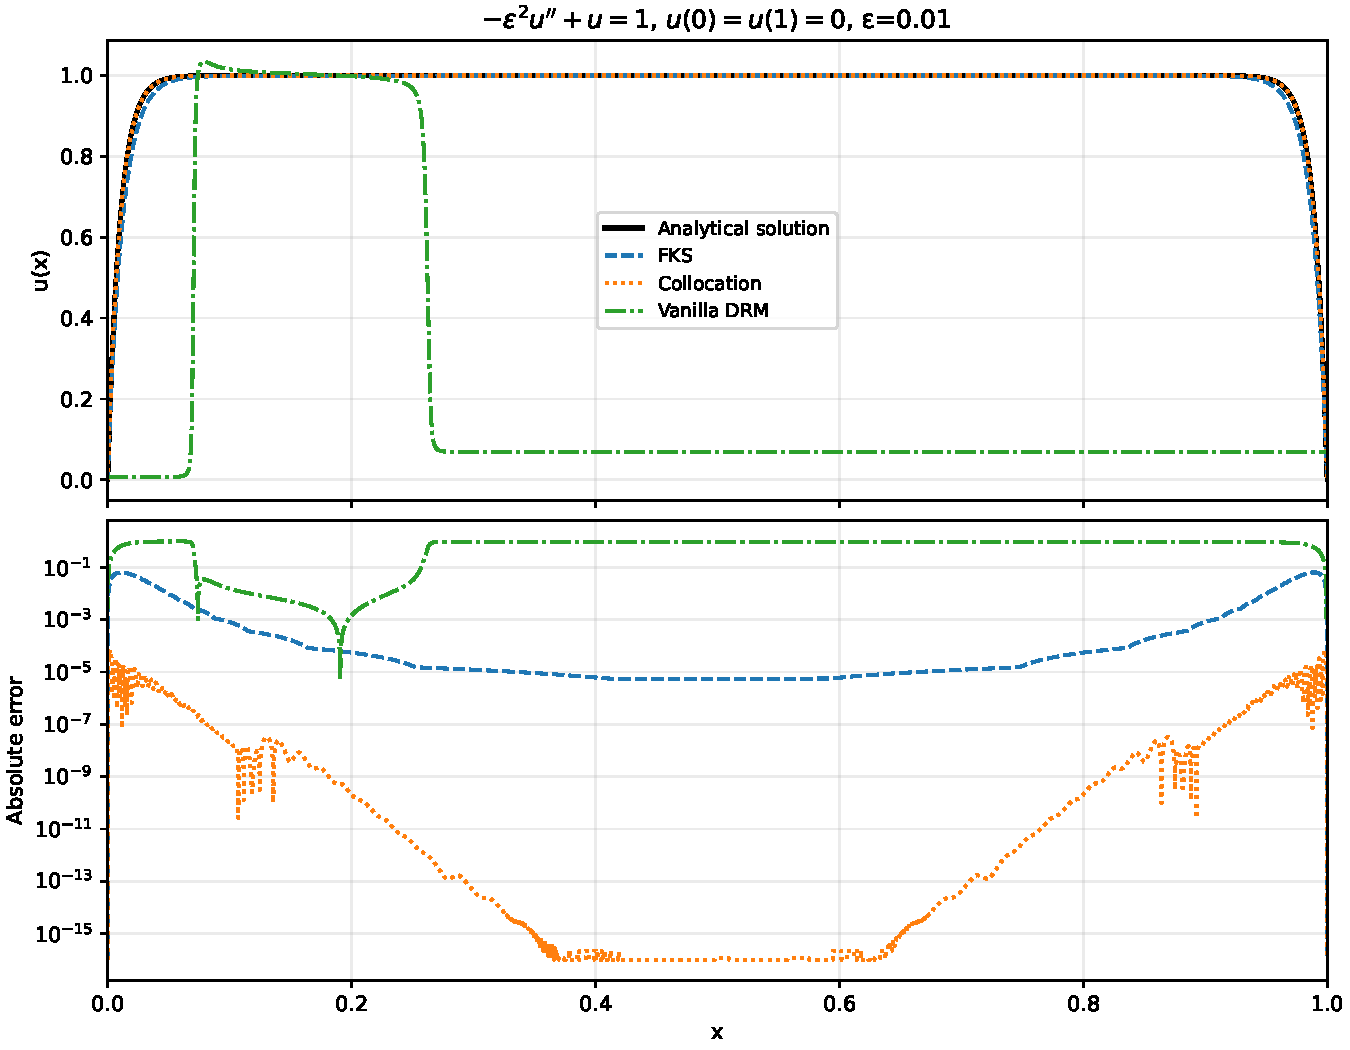
\includegraphics[width=0.8\textwidth]{elliptic_comparison.pdf}
    \caption{Stationary reaction--diffusion problem with
    $\varepsilon=0.01$.
    Top: FKS, collocation and vanilla DRM approximations
    compared with the analytical solution.
    Bottom: pointwise absolute errors.}
    \label{fig:elliptic-comparison}
\end{figure}

We compare the adaptive free-knot spline method (FKS) with vanilla Deep Ritz (DRM) and a collocation solver. Accuracy is measured using the absolute \(L^2\) error, the \(H^1\)-seminorm error and the boundary residual
\begin{equation*}
r_{\partial}=\bigl(|u_h(0)|^2+|u_h(1)|^2\bigr)^{1/2}.
\end{equation*}
Errors are integrated on a common partition containing the spline breakpoints and an independent uniform grid. Increasing the Gauss–Legendre quadrature order from eight to sixteen points per interval changed the errors by less than the prescribed tolerance.

\begin{table}[htbp]
    \centering
    \begin{tabular}{lccc}
        \hline
        Method & $L^2$ error & $H^1$-seminorm error & $r_{\partial}$ \\
        \hline
        FKS         & $1.3158 \times 10^{-2}$ & $1.2633$                  & $1.3878 \times 10^{-17}$ \\
        Collocation & $4.8751 \times 10^{-6}$ & $4.7886 \times 10^{-3}$   & $4.3372 \times 10^{-17}$ \\
        Vanilla DRM & $8.2396 \times 10^{-1}$ & $1.9913 \times 10^{1}$    & $6.9129 \times 10^{-2}$  \\
        \hline
    \end{tabular}
    \caption{Errors for the stationary reaction--diffusion problem
    with $\varepsilon=0.01$, where
    $r_{\partial}=\bigl(|u_h(0)|^2+|u_h(1)|^2\bigr)^{1/2}$.}
    \label{tab:elliptic-errors}
\end{table}

For these runs, FKS reduces the \(L^2\) and \(H^1\)-seminorm errors relative to vanilla DRM by factors of approximately \(1-2\) orders of magnitude. With the FKS architecture, the boundary values can be implemented directly and have been here. This is shown by the boundary residual being of the order of floating point error. The collocation method however, achieves substantially smaller errors than either learned approximation and remains the target for any neural network based solver in 1D. The remaining FKS derivative error indicates that accurate solution values alone do not ensure accurate resolution of the boundary-layer gradients.

\subsubsection{Time Dependant Problem}
We also consider the time dependant version of the problem

\begin{equation*}
    \frac{\partial u}{\partial t} = -\varepsilon^2 \frac{\partial^2 u}{\partial x^2} + u - 1
\end{equation*}

on $[0,1]$, with $\varepsilon=0.01$, homogeneous Dirichlet conditions and initial data $u(x,0)=\sin(\pi x)$. This is solved using the time-stepping method outlined in section \ref{sec:timesteppingMethod}. Figure~\ref{fig:elliptic-time-dependent} compares the FKS approximation with a numerical collocation reference over $0\leq t\leq10$. Both solutions approach unity in the interior while developing boundary layers at the endpoints. The knot trajectories show that the adaptive method concentrates resolution near these layers. The interior knots continue to oscillate due to the lack of control the monitor function has over almost-flat regions. 

The signed-error profiles and error heatmap in Figure~\ref{fig:elliptic-time-dependent} show that the largest discrepancies occur within the boundary layers, where FKS underestimates the reference by approximately $0.1$. The interior error decreases as the solution approaches its stationary profile, but persistent boundary-layer errors cause the $L^2$ and $H^1$-seminorm errors to plateau. The substantially smaller reference-refinement discrepancy in $L^2$ supports using the collocation solution for this comparison. The method therefore captures the overall evolution and concentrates knots in the relevant regions, but does not fully resolve the boundary-layer profiles and gradients at the settings used. 

\begin{figure}[htbp]
    \centering
    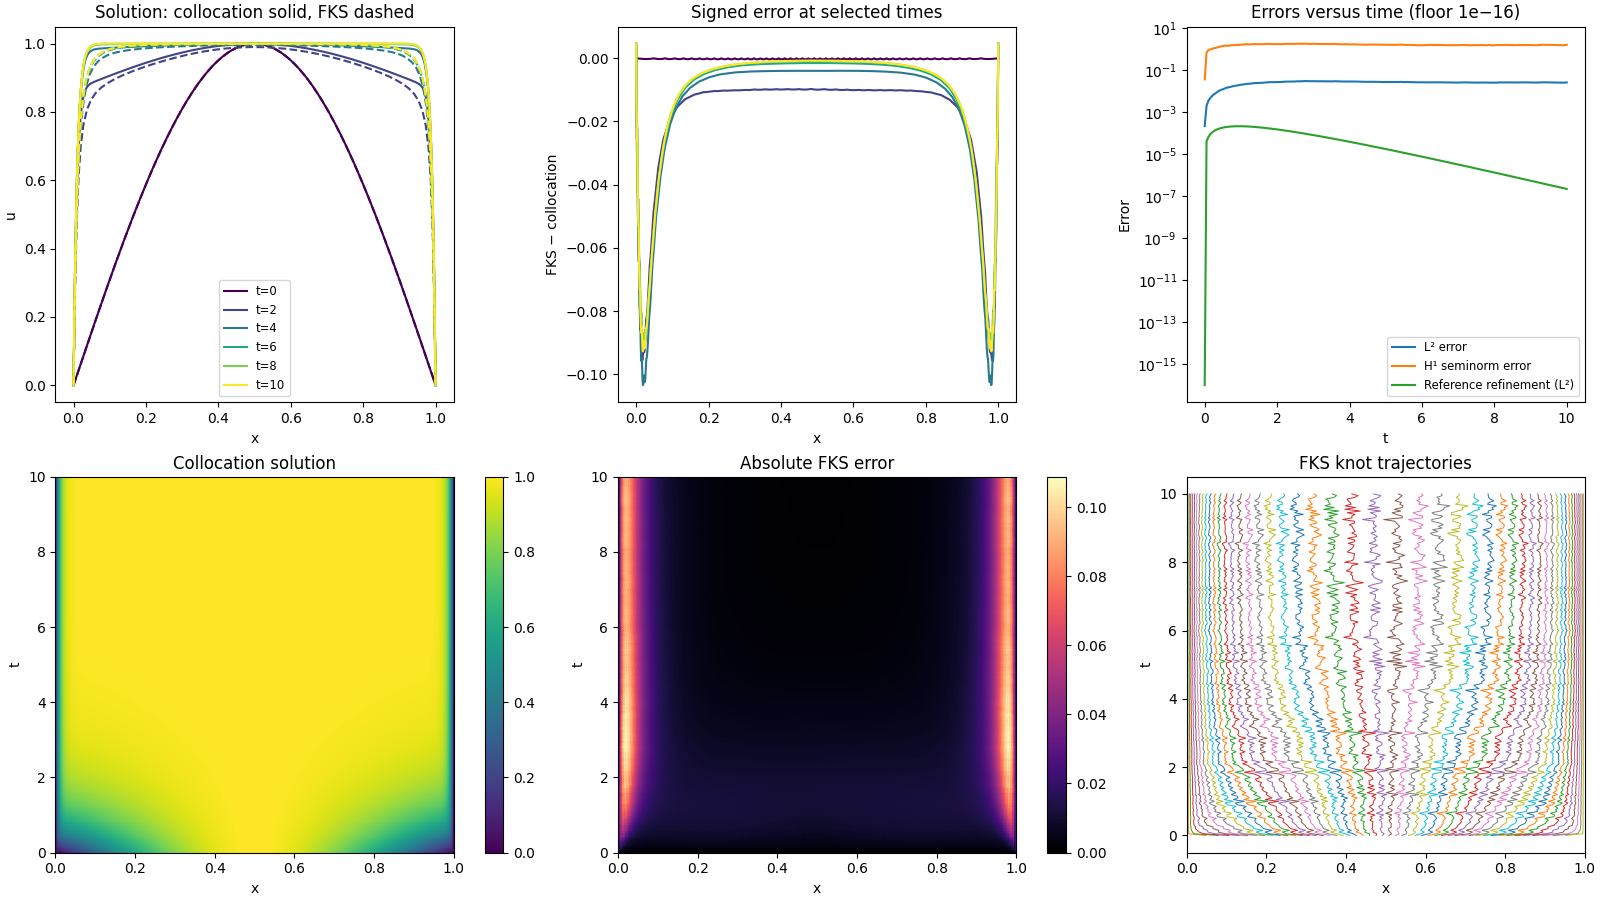
\includegraphics[width=0.8\textwidth]{elliptic_time_dependent.png}
    \caption{Time-dependent reaction--diffusion problem with $\varepsilon=0.01$, homogeneous Dirichlet conditions and initial data $u(x,0)=\sin(\pi x)$. Top row: collocation (solid) and FKS (dashed) solutions at selected times; signed errors; error norms and the $L^2$ reference-refinement discrepancy. Bottom row: collocation solution; absolute FKS error; adaptive knot trajectories.}
    \label{fig:elliptic-time-dependent}
\end{figure}

\subsection{Convection-Diffusion Problem}
We consider the convection--diffusion problem
\begin{equation*}
-\varepsilon u''+u'=1,\qquad x\in(0,1),\qquad u(0)=u(1)=0,
\end{equation*}
with $\varepsilon=0.1$. 
The analytical solution is
\begin{equation*}
u(x)=x-\frac{e^{x/\varepsilon}-1}{e^{1/\varepsilon}-1}.
\end{equation*}
To obtain a variational minimisation problem, we multiply the equation by the integrating factor $e^{-x/\varepsilon}$, giving the energy
\begin{equation*}
E[u]=\int_0^1 e^{-x/\varepsilon}\left(\frac{\varepsilon}{2}(u')^2-u\right)\,dx.
\end{equation*}
This weight decreases by a factor of $e^{10}$ across the domain. Consequently, variations in coefficients associated with localised basis functions near the outflow boundary contribute much less to the objective than comparable variations near the inflow boundary. This disparity can worsen conditioning and slow the optimisation of those coefficients, precisely where the boundary layer requires accurate resolution.

Figure~\ref{fig:convection-comparison} compares the FKS, collocation and vanilla DRM approximations. Both learned approximations capture the initial rise but deviate substantially towards the right boundary.

FKS achieves an $L^2$ error of $5.66\times10^{-2}$, approximately half that of vanilla DRM. However, the corresponding $H^1$-seminorm errors are $1.37$ and $1.51$, respectively, indicating only a modest improvement in derivative accuracy. Exact enforcement of the FKS endpoint values eliminates the boundary residual but does not ensure accurate resolution of the adjacent layer. Collocation is substantially more accurate, with $L^2$ and $H^1$-seminorm errors of $2.05\times10^{-6}$ and $2.68\times10^{-4}$. These results highlight the greater difficulty of the convection--diffusion example: the FKS approximation improves solution values relative to the tested DRM configuration, but significant errors remain in the outflow region. 

\begin{figure}[htbp]
    \centering
    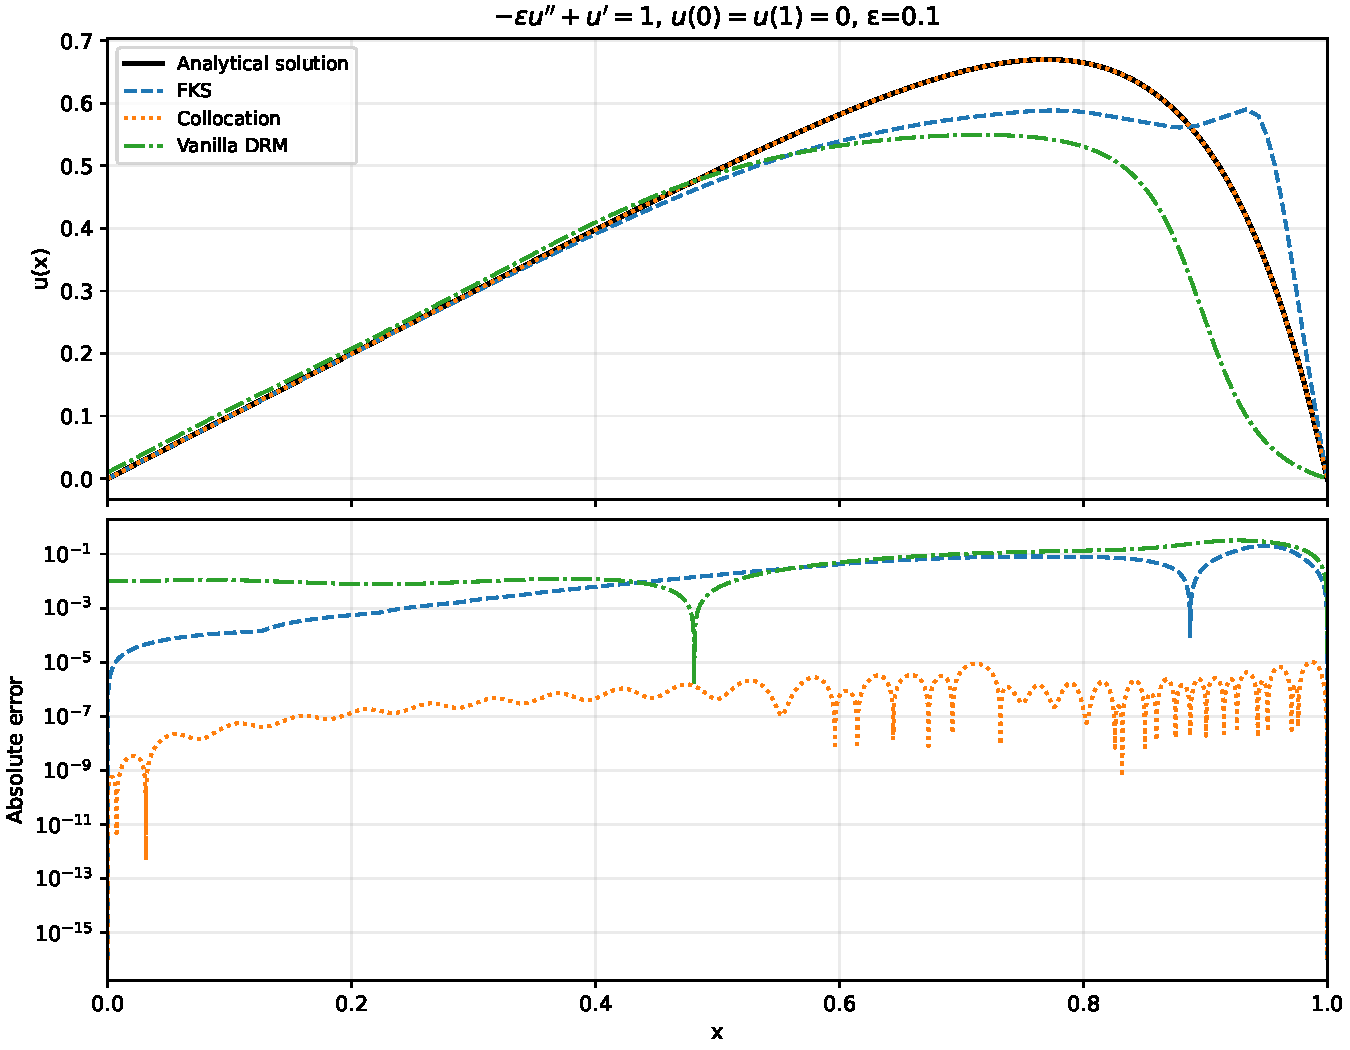
\includegraphics[width=0.8\textwidth]{convection_comparison.pdf}
    \caption{Stationary convection--diffusion problem $-\varepsilon u''+u'=1$, with $u(0)=u(1)=0$ and $\varepsilon=0.1$. Top: FKS, collocation and vanilla DRM approximations compared with the analytical solution. Bottom: pointwise absolute errors.}
    \label{fig:convection-comparison}
\end{figure}

\subsection{Allen-Cahn}
We consider the stationary Allen--Cahn problem
\begin{equation*}
-\varepsilon^2u''+u^3-u=0,\qquad x\in(-1,1),\qquad u(-1)=-1,\quad u(1)=1,
\end{equation*}
with $\varepsilon=0.01$. The reference profile is
\begin{equation*}
u_{\mathrm{ref}}(x)=\tanh\left(\frac{x}{\sqrt{2}\varepsilon}\right),
\end{equation*}
which satisfies the differential equation exactly and the finite-domain boundary conditions to exponentially small error. Unlike the preceding linear problems, the Allen--Cahn energy is non-convex in the represented function, so fixing the knots does not generally make coefficient optimisation convex. The numerical outcome can therefore depend strongly on initialisation. We initialise the FKS nodal values using $u_0(x)=x$ to favour the centred monotone transition. Random initialisation can produce different numerical profiles, although these require separate residual checks before being identified as distinct stationary solutions.

Figure~\ref{fig:allen-cahn-comparison} shows that FKS closely captures the centred transition, whereas vanilla DRM produces a sharper transition displaced towards positive $x$. FKS achieves $L^2$ and $H^1$-seminorm errors of $4.20\times10^{-3}$ and $4.20\times10^{-1}$, compared with $5.39\times10^{-1}$ and $2.90\times10^{1}$ for vanilla DRM. Both approximations have small boundary residuals, indicating that their principal differences occur within the domain rather than at its endpoints. Collocation gives the smallest errors, at $7.0732\times10^{-9}$ and $2.77\times10^{-5}$, respectively. The FKS error is concentrated around the internal layer, highlighting the remaining difficulty of resolving its steep gradient even when the transition is correctly located.

\begin{figure}[htbp]
    \centering
    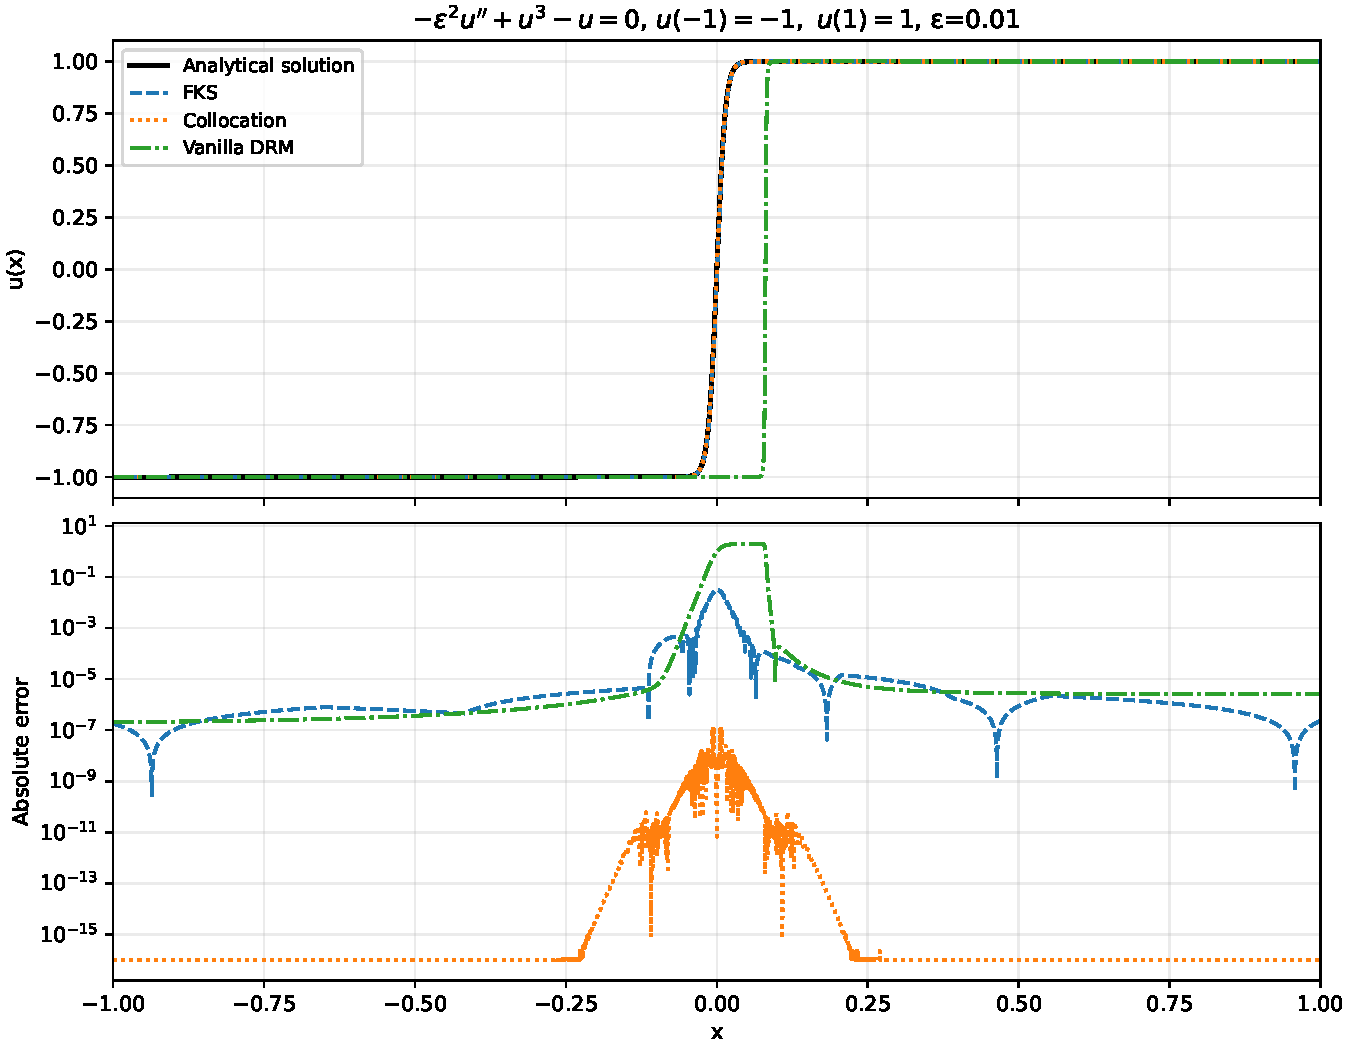
\includegraphics[width=0.8\textwidth]{allen_comparison.pdf}
    \caption{Stationary Allen--Cahn problem $-\varepsilon^2u''+u^3-u=0$, with $u(-1)=-1$, $u(1)=1$ and $\varepsilon=0.01$. Top: FKS, collocation and vanilla DRM approximations compared with the reference profile $\tanh(x/(\sqrt{2}\varepsilon))$. Bottom: pointwise absolute errors.}
    \label{fig:allen-cahn-comparison}
\end{figure}

\subsubsection{Time Dependant Problem}
Finally, we consider the time dependant variant of the Allen-Cahn problem given by 

\begin{align*}
    \frac{\partial u}{\partial t}(x,t)
    - \varepsilon^2 \frac{\partial^2 u}{\partial x^2}(x,t)
    + u(x,t)^3 - u(x,t) &= 0,
    && x\in(-1,1),\quad t\in(0,T], \\[10pt]
    u(-1,t)=u(1,t) &= 0,
    && t\in[0,T], \\
    u(x,0) &= u_0(x),
    && x\in[-1,1].
\end{align*}

where different $u_0$ are chosen to specify different behaviours. 




\chapter{Current Research}
\label{chap:CurrentResearch}
\section{Eigenvalue Problems on Complex Domains}
\label{sec:Eigenvalue}
\section{2D PINNs and DRM - Conditioning and Expressivity}
\label{sec:Conditioning}

\chapter{Future Work/Research}
\label{chap:FutureResearch}
\section{Paper Submission}
The paper outlined in chapter \ref{chap:Paper} will likely go through one or more revisions before it is ready to be published. The aim is to complete this over the course of the next two months with advice from other academics within the Mathematics department. This may be extended if for example more test problems are included or a sensible line of research is suggested. 


\section{Case for convergence: Optimal warm start for time--dependant PDEs}
\label{sec:WarmStart}

A recent idea for a research direction has come off the back of the time-dependant solutions in chapter \ref{chap:Paper}. These methods often perform better than their time independent counterparts due to the initial data acting as a good initialisation of the neural network. Explicitly for the FKS model, this initialisation is near optimal due to the shallow nature of the network. 

To generalise this, starting with the optimal neural network representation of an initial condition $u_0 = u(x,0)$ which we denote $\hat u_\theta^0$. The parameters $\theta_*^0$ that give us this initialisation exist as a global minima for the PINN/DRM loss function at time-step 0 and more importantly exist within the ``basin of attraction" (i.e. within a domain corresponding to a convex optimisation problem to find the global minima). 

With a sufficiently small time step, the evolution of this loss function should mean that using the parameters $\theta_*^0$ as our initialisation for time step t=1 should remain within the ``basin of attraction'' for the global minima for this time step.

This argument can be followed through for future timesteps and may potentially allow us to reduce the convergence argument for time-stepped PDEs down to that of optimally training for initial conditions. There likely remain some issues with this argument, such as those of competing global minima but these can be investigated as part of the future research.

This therefore highlights some questions worth answering:

\begin{itemize}
	\item Given a fixed architecture, can one find the optimal network representation for a known function u(x)?
	\item How do global minima of PINN/DRM loss functions evolve under time stepping methods such as implicit euler or Crank-Nicolson?
\end{itemize}


\section{Proving general NN based methods cannot guarantee convergence}
\label{sec:Proof}

From experimental evidence, without an initialisation which initialised a GD based methods within the ``basin of attraction'' of the global minima for a PINN loss function, I believe that it is unlikely one can use local methods to discern the global minima and therefore guarantee convergence to within an arbitrary error bound. This is predominantly due to the fact that the loss function is explicitly dependant on the neural network architecture which as a non-linear function will likely cause the loss landscape to be non-convex. 

I believe it is worth formalising the sentiment expressed here as something along the lines of ``Gradient Descent based methods cannot guarantee convergence of a deep neural network based PDE solution approximation to within an arbitrary error tolerance of the solution to the PDE''.
 This research has merit due to its ability to be abstracted to a larger class of neural network based problems and shifts the discussion from trying to guarantee perfect accuracy within scientific machine learning to identifying cases that minimise the chance of approximation error. One such example of this within the PINNs setting is that of Variationally Boosted PINNs \cite{BoostedPINNs} which produces a solution approximation as the linear combination of multiple smaller neural networks in place one one larger neural network with the same total number of parameters. In doing so, the architecture is smaller and therefore provides a reduced parameter space to explore, increasing the chance of discovering the global minima.


\section{Optimal tradeoff between expressivity and conditioning}
Following on from the research proposed in section \ref{sec:Proof}, a sensible follow up question might be to ask what the optimal architectural choice is to minimise the chance of optimisation failure whilst keeping the expressivity quality of deep neural networks. This directly follows on from the current research on conditioning and expressivity in chapter \ref{chap:CurrentResearch} section \ref{sec:Conditioning} and pitches it in a broader setting asking questions about alternate architectures and a wider scope of problem than PDEs in two spatial dimensions.

\chapter{Doctoral Training}
This chapter outlines my professional outside of performing research. It includes tutoring, teaching, conferences and workshops, seminars, research group events, and departmentally run events.

\section{Tutoring}
During my PhD I have tutored undergraduate mathematics students as a Graduate Teaching Assistant. I have tutored for the Multivariable Calculus (MVC) (MA12002) and Vectors, Vector Calculus and Mechanics (MA12003) courses with two classes per semester for the last four semesters.

 I am currently in the process of submitting my application to be  Associate Fellow of the Higher Education Association (AFHEA). \cite{AFHEA} This requires evidencing a ``personal and institutional commitment to professionalism in learning and teaching in higher education.'' across a multitude of highlighted areas. To do this I have analysed and experimented with my tutoring to better understand how to communicate mathematics at a higher education level effectively and have played an active part within the Mathematics tutoring community at the University of Bath. This includes attending PRIME seminars on mathematics education, attending supplementary training on tutoring and aiding new tutors within the department. I also bake for my tutees. 
 
\section{SciML for KEHub}
Over the last year Professor Chris Budd and I have developed and delivered an introduction to Scientific Machine Learning course predominantly aimed at those who are aware of but have not yet interacted with the world of SciML. This includes individuals from industries such as telecommunications, technology, biotech and more and those from mathematically adjacent academic settings such as Physics and Engineering. The course is based off of our research into the field with an introduction to PINNs and the DRM directly based upon research outlined earlier in this report. The course is a day long event with 4 lectures and a coding workshop delivered online through teams and google colab. I have been responsible for delivering the PINNs/DRM lecture and running the workshop at the end of the day.

Alongside this we have turned this course into a miniature handbook/textbook which acts as an introduction to SciML in an easily digestible format. This handbook is currently going through the editorial process and will hopefully be published before the end of the year.

\section{Conferences, Workshops, and Seminars}
During my PhD I have so far attended 3 conferences and 1 workshop. The workshop was a week long SciML focused event for early career academics held at the CWI in Amsterdam. Chris and I delivered a variant of the SciML course at this workshop introducing these researchers to PINNs, the DRM, Neural Operators and NeuralODEs alongside running the coding lab at the end of the day. The workshop also ran days focused on diffusion modelling, inverse problems and data assimilation, JAX, and back-propogation.

Of the three conferences I have attended, I have presented the research documented in chapter \ref{chap:Paper} at two of them. Initially at the REMODEL conference in Trondheim in May 2026 and then again at SciCADE 2026 in Edinburgh. I recently attended the SCML 2026 workshop at the University of Bath but did not present any work at this time.

I regularly attend the Numerical Analysis and Data Science (NA+DS) and Practice and Research in Mathematical sciences Education (PRIME) seminars within the Mathematics Department. Alongside this I also occasionally attend the AIMS and CAI seminars when my timetable and research interests allow. I have also presented work at the student led PSS (postgraduate seminar series) as practice for presenting at conferences. 

\section{Departmental Training, Study Groups, and Hackathons}
Twice a year the department runs Integrated Think Tanks which I have attended all of since joining SAMBa. These are week long events where researchers in the department (predominantly PhD students) act as mathematical consults for industrial partners with the aim of formulating research questions based on industrial interests. I have worked with BT, Novartis, University of Bath Department of Life Sciences and the National Grid during my attendance covering a range of mathematical fields including statistical modelling (FDA), NeuralODEs, Inverse Problems and Stochastic Modelling.

I have also attended training days on Responsible Research and Innovation (RRI) and other departmental training. 

Similar to the ITTs, I have taken part in an European Study Group for Industry (ESGI) where I worked with CameraForensics (a Bristol based cyber security company) working on automatically identifying when Generative models had been trained on illegal content. 

I have also attended a Hackathon which was run at the University of Cambridge in partnership with the National Air Traffic Services (NATS) investigating ML application to air traffic management. 

\section{Personal Development}
Separately from my work at the university, I run a local scout group in Bath as a way to give back to the local community. During my time there I have completed my Kings Scout Award - the highest award available within scouting and am currently in the process of making sure the group is in a stable position for when I leave in 2 years time.

\chapter{Research Timeline}
Here I outline upcoming events, research goals and trips within the next twelve months (Oct '27 inclusive) in chronological order. 
\begin{itemize}
	\item Oct '26 -- \textbf{AHFEA Application Submission}: This is predominantly written and requires a small polish before submission next month.
	
	\item Nov '26 -- \textbf{Bath Taps into Science}: Similar to last year, I aim to help out at Bath Taps into Science with the Maths department. This is an annual outreach event aimed at late primary/early secondary aged students. 
	
	\item Nov '26 -- \textbf{Visit to Parliament for annual Parliamentary Maths Expo}: I am attending this alongside other members of the M4DL group to lobby politicians on the need for SciML and wider applied mathematics funding. 
	
	\item Nov '26 -- \textbf{Finish and submit paper in chapter \ref{chap:Paper}}: The paper presented in chapter \ref{chap:Paper} will likely go through another couple of drafts before submission. The aim is to have this finished by the end of November.
	
	\item Dec '26 -- \textbf{Police VSG}: I plan to attend a virtual study group in collaboration with the NPCC and P-ACE working on data heavy problems.
	
	\item Jan '27 -- \textbf{Condition Number Estimates}: The first research goal in the timeline focusing on completing work outlined in chapter \ref{chap:CurrentResearch}. section \ref{sec:Conditioning}. I aim to have strong experimental evidence for condition numbers and an estimate for how the tradeoff between expressivity and conditioning looks like for these problems.
	
	\item Jan '27 -- \textbf{Optimal Architecture}: Following on from the previous point. The next aim is to identify an optimal architecture for a given problem.
	
	\item Early '27 -- \textbf{NN Representation of known functions}: This research checkpoint represents work completed for the direction outlined in chapter \ref{chap:FutureResearch} section \ref{sec:WarmStart}. To prove a convergence theory in the setting outlined here, one would need an optimal neural network representation of the initial conditions in a time dependant problem. Regardless of whether this direction ends up being successful, I believe that this is a useful mathematical subproblem to investigate - hence its own research checkpoint.
	
	\item Mid '27 -- \textbf{Optimal Architecture Paper}: The culmination of the current work being completed in chapter \ref{chap:CurrentResearch} section \ref{sec:Conditioning}. The aim is to have this paper written by mid 2027.
	
	\item May '27 -- \textbf{REMODEL Simon Fraser University visit}: Through the REMODEL grant I plan to visit Professors Nilima Nigam and Ben Adcock at Simon Fraser University for a month around May 2027. Here I plan to continue my research and potentially identify new research directions to go in.
	
	\item May '27 -- \textbf{Eigenvalue Problem Progression}: Using my time in Vancouver as a checkpoint. I hope to have made progress on the current work outlined in chapter \ref{chap:CurrentResearch} section \ref{sec:Eigenvalue}. I will use my time with Professor Nigam to further this research as well.
	
	\item July '27 -- \textbf{Leiden Workshop/ICIAM}: In July 2027 I plan to attend the International Congress for Industrial and Applied Mathematics (ICIAM) in the Hague. My supervisor, Professor Chris Budd, is an invited speaker for this event. The week before this, there is a week long workshop in SciML being held at Leiden University which we also both plan to attend.
	
	\item Sept '27 -- \textbf{SCML Trondheim}: I plan to attend SCML 2027 in Trondheim as this is a conference directly related to my research and I am familiar with the research community who will be presenting here. Depending on the work I have completed I aim to present at this conference. 
	
	\item Sept/Oct '27 -- \textbf{REMODEL Kyushu University visit}: Similar to my visit to SFU, I plan to visit Professor Takaharu Yaguchi at Kyushu University in Fukuoka, Japan in autumn 2027. This will be funding dependant but again I would spend a month there looking for new research directions. Takaharu's group has a strong focus on structure preserving ML and Neural Operators so I may look to ask similar convergence questions of these methods to those I have asked of PINNs.  
	
	\item Late '27 -- \textbf{PINNs Proof}: This is a research checkpoint focusing on the work outlined in chapter \ref{chap:FutureResearch} sections \ref{sec:WarmStart} and \ref{sec:Proof}. I see this as the definitive end to the research question asked in the introduction and would like to have an answer to this by the end of next year.
	
	\item Nov '27 -- \textbf{Bath Taps into Science}: The same as the '26 edition. I plan to help out here again.
	
\end{itemize}

\bibliography{ref}
\bibliographystyle{unsrt}


\end{document}
